% Предустановленные пакеты:
%   texlive-full
% Команда для сборки:
%   latexmk -pdf -bibtex -latexoption="-file-line-error -synctex=1 -interaction=nonstopmode -shell-escape" $fullname

\documentclass[10pt]{geodmanual}

\title{Гравиметр CG-6 Autograv\texttrademark{}}

\orgFullName{}
\orgShortName{}
\divName{}
\depName{}
\manualVersion{C}

\manualType{Инструкция по эксплуатации}
\manualYear{2022}
\manualCity{Астана}
\def \pathtotitlepic {figures/cg6_title.png}

\includeonly{
  chapters/instrument_overview,
  chapters/getting_started,
  chapters/setting_up_your_cg6_autograv,
  chapters/operating_the_cg6_autograv_in_the_field,
  chapters/maintenance_and_troubleshooting,
  chapters/reference_information,
}

%\manualVersion{\ShowRepoVersion}


\begin{document}

\newcommand{\cg}{CG-6 Autograv\texttrademark{}}

\maketitle
\tableofcontents

\chapter[Обзор]{Обзор прибора}
\label{chap:instrument_overview}

\begin{figure}[h]
  \centering
  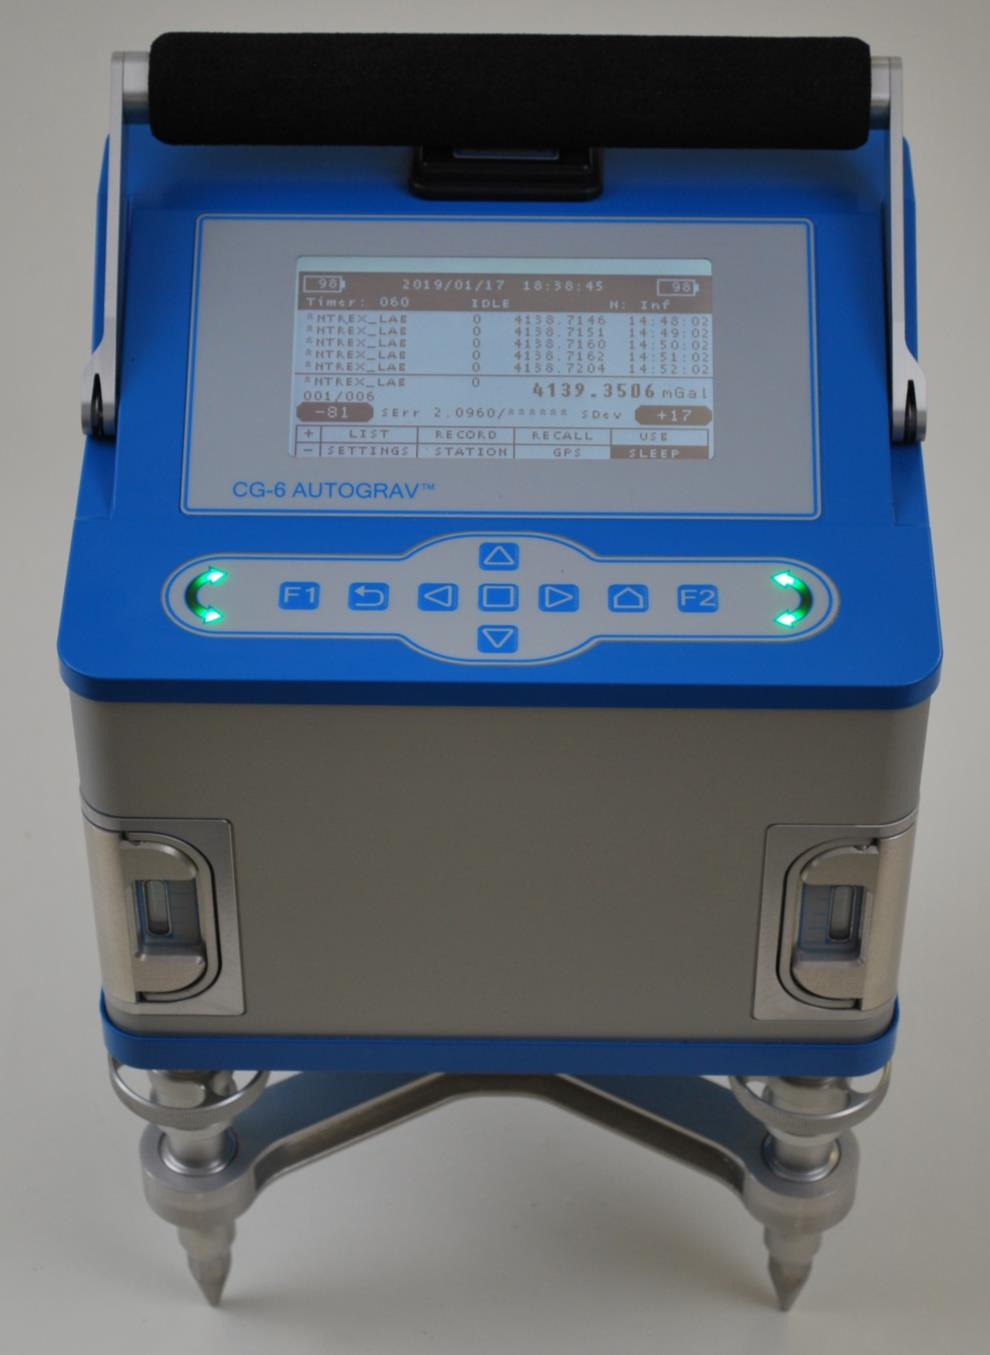
\includegraphics[width=0.9\textwidth, height=0.5\textheight, keepaspectratio]
  {figures/cg6_autograv}
  \caption{Гравиметр \cg{}}
  \label{fig:cg6_autograv_gravity_meter}
\end{figure}

\cg{}~-- это автоматический гравиметр, способный выполнять измерения в любой
точке мира с разрешением 0,0001 мГал в диапазоне 8000~мГал. Прибор позволяет
проводить как детальные микро гравиметрические измерения, так и крупномасштабные
региональные геодезические исследования.

Измерение выполняется простым нажатием клавиши, и в большинстве случаев процесс
измерения занимает менее одной минуты. Предусмотрена возможность выбора
дополнительных информационных циклов. \cg{} выполняет измерения,
обрабатывая непрерывную последовательность отсчётов длительностью 0,1 секунда.
Измерение вместе с выбранными внесёнными поправками отображается на ЖК-дисплее
непосредственно в мГал. Полученные данные сохраняются в памяти прибора, откуда
можно произвести их экспорт в любое удобное время.

Гравитационный датчик, электронные схемы и аккумуляторные батареи размещаются
внутри корпуса прибора.

Для защиты от изменений внешней температуры и атмосферного давления
чувствительные элементы \cg{} помещены в герметичную
термостабилизированную камеру. Благодаря широкому диапазону рабочих
температур~-- от \textminus{}40\textcelsius{} до +45\textcelsius{}~-- систему
\cg{} можно использовать в самых разных условиях окружающей
среды. Предлагается также версия прибора для высокотемпературных районов с
диапазоном рабочих температур от \textminus{}40\textcelsius{} до
+55\textcelsius{}.

Встроенные датчики наклона предоставляют системе \cg{}
информацию об угле наклона~-- это позволяет в режиме реального времени вводить
поправки в результаты измерений, выполняемых на неустойчивом грунте.

Горизонтирование прибора \cg{} не представляет сложности,
благодаря наличию двух стрелок со светодиодной подсветкой на панели прибора. Эти
стрелки показывают оператору направление, в котором нужно вращать винты штатива.

Две встроенные перезаряжаемые Li-ионные аккумуляторные батареи обеспечивают
систему \cg{} достаточной энергией питания для работы в
течение стандартного дня съёмки.

Внешний планшетный компьютер позволяет оператору легко настраивать рабочие
параметры системы \cg{} и сохранять эти настройки, а также
планировать и сохранять пункты съёмки. Планшетный компьютер поставляется с
установленным программным обеспечением LynxLG Land Gravity, с помощью
которого оператор может планировать предстоящую съёмку, осуществлять
удалённые измерения и непрерывный мониторинг сигналов силы тяжести и угла
наклона. Помимо прочих разнообразных функций планшетного компьютера, можно
отметить доступ к картам.

Если эксплуатация системы осуществляется при температуре окружающей среды ниже
\textminus{}20\textcelsius{}, рекомендуется использовать комплект
принадлежностей (номер 888405) для холодной погоды.

Среди других имеющихся принадлежностей~-- рюкзак Seco (\textnumero{}~140220) и
штатив для измерения градиента (No 101370004).

\chapter[Начало работы]{Начало работы}
\label{chap:getting_started}

\section{Главы и их содержание}

\begin{table}[h]
  \begin{tabulary}{\textwidth}{|L|L|}
    \hline
    Глава & Описание \\
    \hline
    1. Обзор & Описание прибора \\
    \hline
    2. Начало работы & Знакомство с руководством и описание составных частей
    прибора \\
    \hline
    3. Подготовка к работе & Подготовка вашего прибора CG-6
    Autograv\texttrademark{} к проведению съёмки \\
    \hline
    4. Эксплуатация & Эксплуатация прибора \cg{} при
    проведении съёмки \\
    \hline
    5. Техническое обслуживание & Как проводить техническое обслуживание и
    устранять неполадки в приборе \cg{} \\
    \hline
    6. Справочная информация & Технические характеристики, спецификация деталей
    прибора, и сведения о гарантии \\
    \hline
  \end{tabulary}
\end{table}

\section{Условные обозначения}

\warningbox{
  Содержится указание на важный предмет обсуждения, этому разделу нужно уделить
  особое внимание
}

\infobox{
  Акцентируется внимание на информации, представляющей особый интерес для
  пользователя
}

Необходимые для выполнения действия, такие как <<нажать>>, <<ввести>> и
<<редактировать>>, выделяются \textit{курсивом}. Кнопки клавиатуры выделяются
\textbf{жирным шрифтом}. Пункты меню выделяются заглавными буквами и
\textbf{ЖИРНЫМ ШРИФТОМ}.

\section{Распаковка прибора}

Прибор \cg{} упакован в кофр с мягкими вставками (при
этом, аккумуляторные батареи располагаются отдельно, в индивидуальной упаковке,
в соответствии с правилами безопасности на транспорте IATA), которые
обеспечивают защиту прибора во время доставки и перевозки.

\warningbox{
  Перевозка прибора должна осуществляться с извлечёнными аккумуляторными
  батареями. Батареи должны размещаться отдельно. Если вы только что получили
  прибор \cg{}, имейте в виду, что аккумуляторные
  батареи упакованы отдельно, и заряжены примерно на 30\% от номинального
  объёма.
}

\begin{figure}%[]
  \centering
  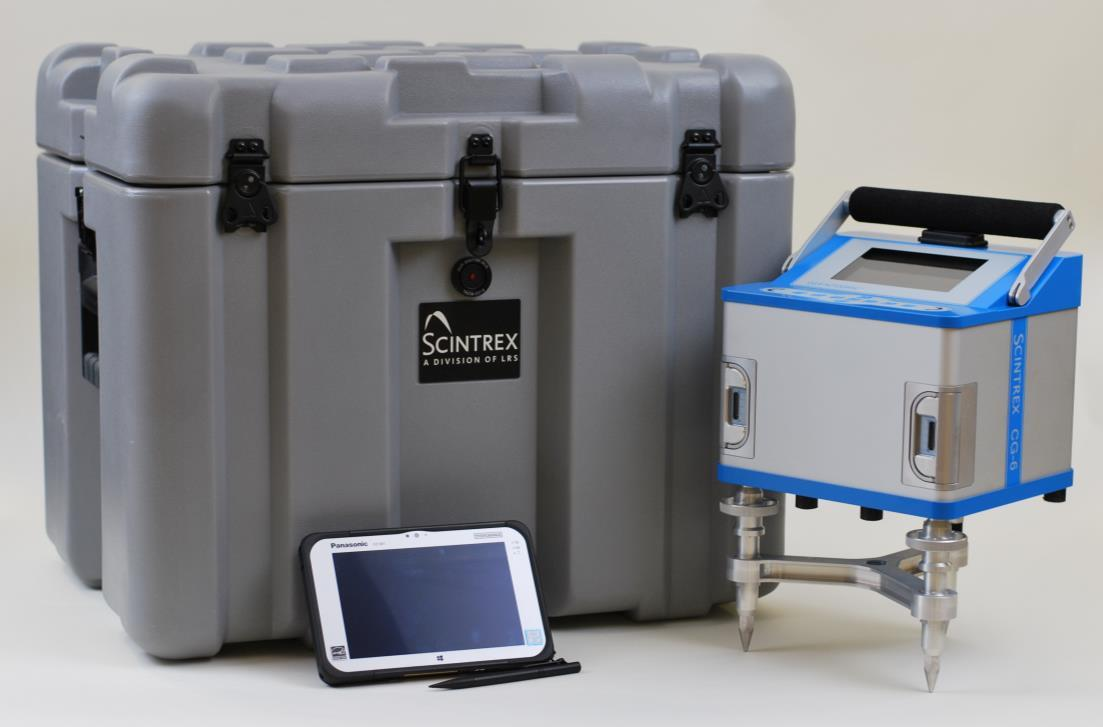
\includegraphics[width=\textwidth]{figures/the_cg6_autograv_gravity_meter_and_its_transportation_case}
  \caption{Гравиметр \cg{} и транспортировочный ящик}
  \label{fig:the_cg6_autograv_gravity_meter_and_its_transportation_case}
\end{figure}

\begin{enumerate}
  \item Надавите на красный клапан сброса избыточного давления, расположенный на
    передней стороне транспортировочного кофра.

  \item\label{item:turn_back} Откиньте вверх язычок фиксатора и поверните язычок против часовой
    стрелки, чтобы фиксатор отсоединился от запорной планки.

  \item Повторите действия по п.~\ref{item:turn_back} для других фиксаторов.

  \begin{figure}[h]
    \centering
    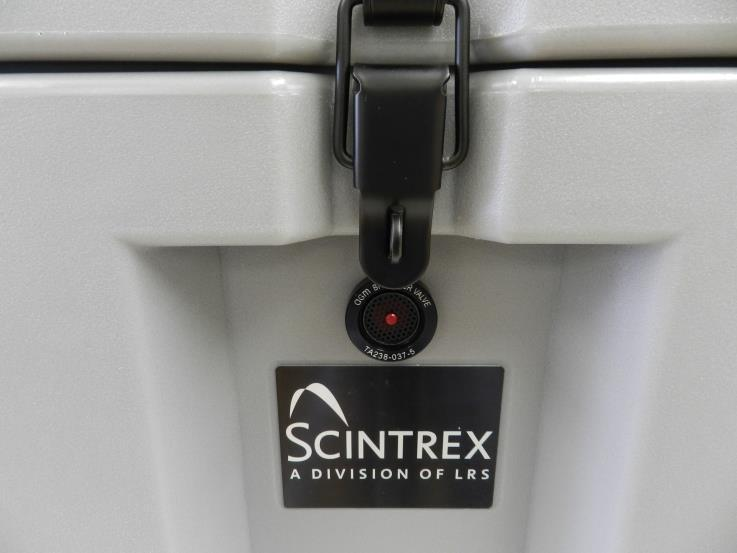
\includegraphics[width=0.7\textwidth]{figures/location_of_the_pressure_release_value_on_the_transportation_case}
    \caption{Клапан сброса избыточного давления на кофре}
    \label{fig:location_of_the_pressure_release_value_on_the_transportation_case}
  \end{figure}

  \item Откройте транспортировочный кофр прибора CG-6
    Autograv\texttrademark{}, подняв крышку.

  \item Извлеките прибор \cg{} из транспортировочного
    кофра, потянув его вертикально вверх за чёрную резиновую ручку. Произведите
    визуальный осмотр прибора на наличие физических повреждений, которые могут
    быть получены во время транспортировки.
\end{enumerate}

\warningbox{
  Транспортировочный кофр прибора CG-6 Autograv\texttrademark{} снабжён
  индикатором удара Shockwatch, который закреплён на боковой стенке.  Проверьте
  индикатор, и если вы обнаружите, что контрольный элемент окрашен в красный
  цвет, немедленно обратитесь в компанию Scintrex Limited.  Обратитесь к разделу
  \nameref{sec:shipping_instructions} на
  странице~\pageref{sec:shipping_instructions}.
}

\begin{figure}%[]
  \centering
  
\includegraphics[width=0.7\textwidth]{figures/shockwatch_monitor}
  \caption{Индикатор удара Shockwatch}
  \label{fig:shockwatch_monitor}
\end{figure}

\section{Обзор составных частей}

На следующем рисунке показан вид сверху всех компонентов, которые поставляются
со стандартной комплектацией \cg{} в транспортировочном
кейсе.

\begin{figure}%[]
  \centering
  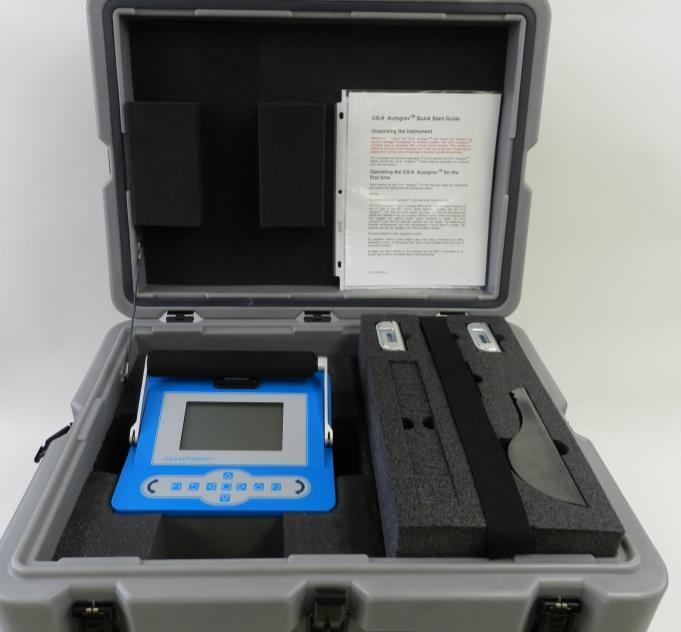
\includegraphics[width=0.7\textwidth]{figures/the_cg6_autograv_and_its_components}
  \caption{Прибор \cg{} и его составные части}
  \label{fig:the_cg6_autograv_and_its_components}
\end{figure}

\section{Обзор панели управления и клавиатуры}

На рисунке~\ref{fig:the_cg6_autograv_console} изображена передняя панель
прибора. Она состоит из дисплея, антенны GPS/Bluetooth, модуля клавиатуры, для
управления прибором и светодиодных стрелок для нивелирования.

\begin{figure}%[]
  \centering
  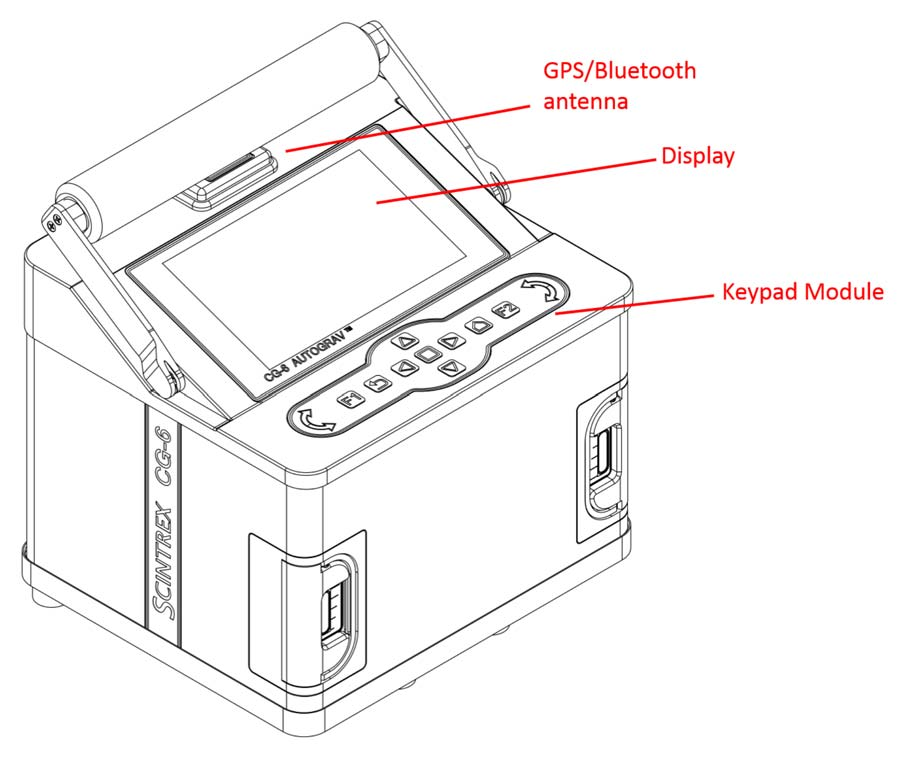
\includegraphics[width=0.7\textwidth]{figures/the_cg6_autograv_console}
  \caption{Панель управления прибора \cg{}}
  \label{fig:the_cg6_autograv_console}
\end{figure}

\begin{figure}%[]
  \centering
  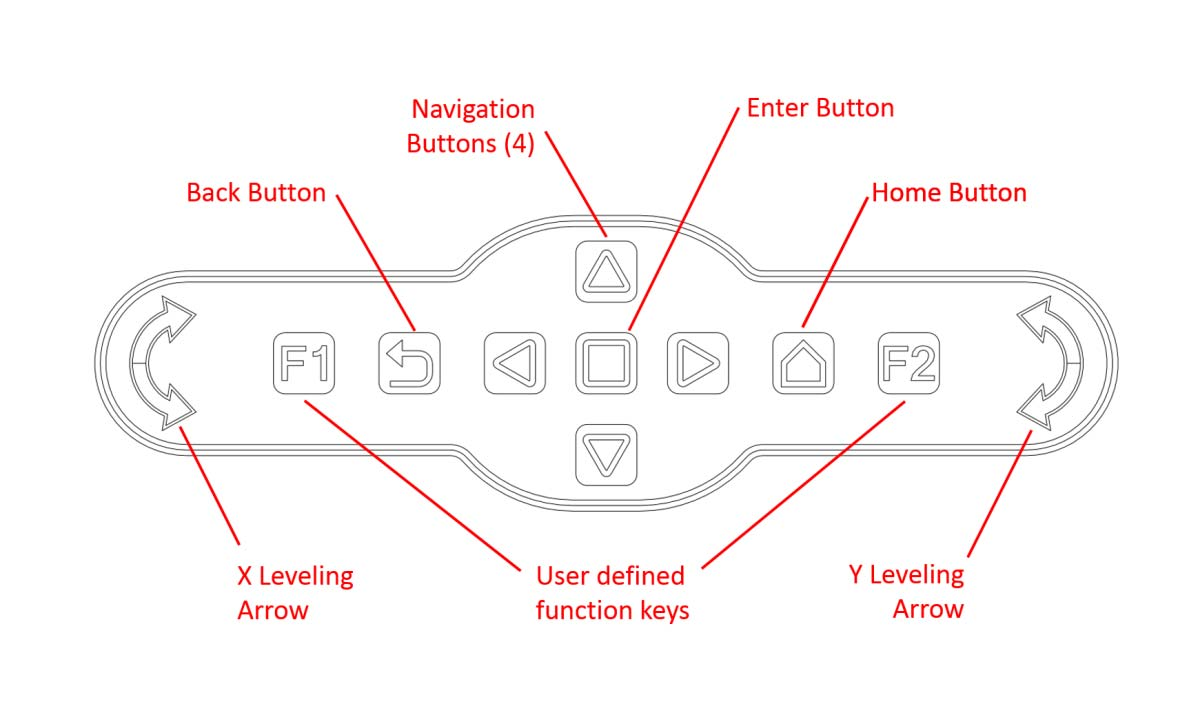
\includegraphics[width=0.7\textwidth]{figures/the_cg6_autograv_keypad_module}
  \caption{Модуль клавиатуры CG-6 Autograv}
  \label{fig:the_cg6_autograv_keypad_module}
\end{figure}

Две стрелки указывают направление, в котором нужно вращать нивелировочные винты
для выравнивания треноги. Стрелка слева относится к левому нивелировочному
винту, а стрелка справа~-- к правому нивелировочному винту.  Правый винт
выравнивает прибор одновременно по осям X и Y, тогда как левый винт выравнивает
прибор только по оси X.

\infobox{
  Хотя для грубого выравнивания можно вращать оба винта штатива одновременно,
  для точного выравнивания может оказаться более эффективным сначала правым
  винтом отрегулировать уровень по оси Y, после этого левым винтом
  отрегулировать уровень по оси X.
}

Вы можете перемещаться между элементами меню, расположенными в нижней части
экрана, используя \textbf{кнопки Navigation} <<Навигация>>, \textbf{Home} <<На
главный экран>>, \textbf{Back} <<Назад>>, \textbf{F1} и \textbf{F2}. На любом
экране переместите курсор либо на \textbf{BACK}, либо на \textbf{CANCEL} и
нажмите кнопку \textbf{Enter}, либо нажмите кнопку \textbf{Back}, чтобы
вернуться к предыдущему экрану. Нажмите кнопку Home, чтобы перейти на главный
экран.

\section[Ввод в работу]{Ввод в работу прибора \cg{}}

Если прибор \cg{} включается в первый раз, или если он
был выключен более 24 часов, необходимо выполнить следующие действия, соблюдая
определённые периоды ожидания.

\paragraph[Подача питания]{Подача питания на прибор \cg{}:} обратитесь к расположенному ниже
разделу под заголовком: \nameref{subsec:powering_up_the_cg6_autograv}

\paragraph{Период прогревания:} после подачи питания на прибор \cg{}{}, время,
необходимое для достижения рабочей температуры, составляет примерно один час.

\paragraph{Период стабилизации:} после подачи питания на прибор требуется 24
часа на его стабилизацию.

\paragraph{Подготовка прибора для полевых работ:} по завершении периода
стабилизации, ваш прибор \cg{} готов к работе.
Обратитесь к следующей главе (Настройка \cg{}), где
содержится подробная информация о подготовке прибора к работе.

\subsection[Подача питания]{Подача питания на прибор \cg{}}
\label{subsec:powering_up_the_cg6_autograv}

Подачу питания на прибор \cg{} можно осуществлять одним
из следующих способов:
\begin{itemize}
  \item От внешнего источника постоянного тока напряжением 15В.

    \begin{figure}[h]
      \centering
      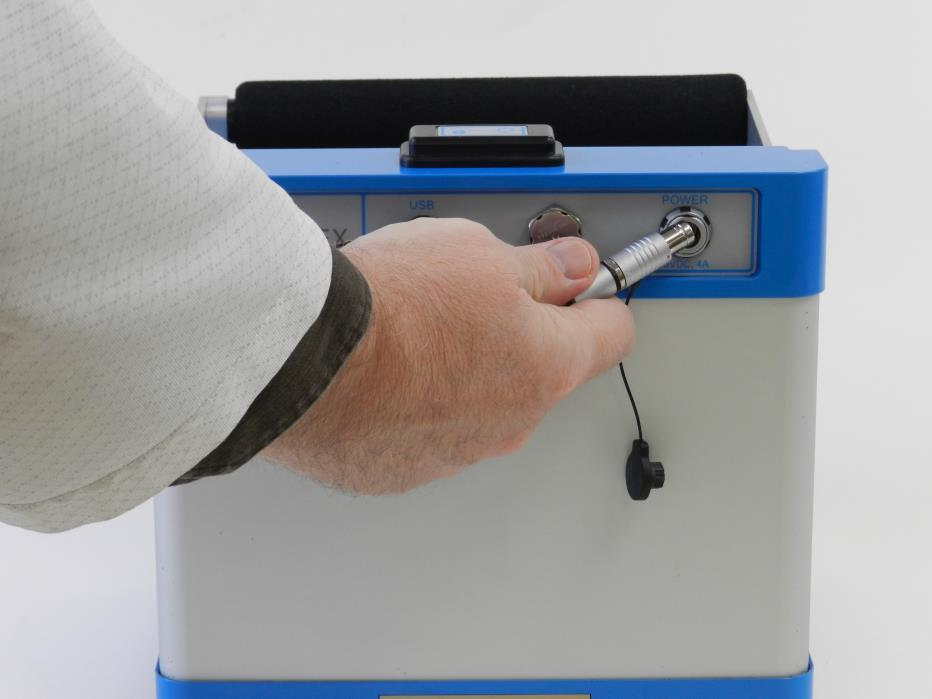
\includegraphics[width=0.7\textwidth]{figures/connecting_the_power_supply_to_the_cg6_autograv}
      \caption{Подключение внешнего источника питания к \cg{}}
      \label{fig:connecting_the_power_supply_to_the_cg6_autograv}
    \end{figure}

  \item От двух встроенных интеллектуальных аккумуляторных батарей, которые
    поставляются вместе с прибором \cg{}.

    \begin{figure}[h]
      \centering
      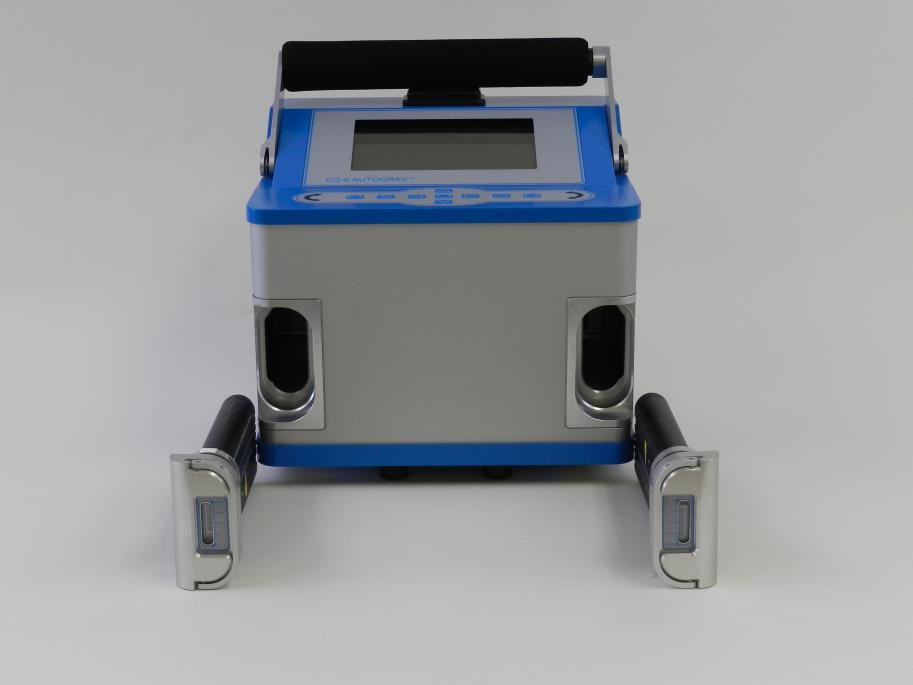
\includegraphics[width=0.7\textwidth]{figures/the_cg6_autograv_and_batteries}
      \caption{Прибор \cg{} с аккумуляторными батареями}
      \label{fig:the_cg6_autograv_and_batteries}
    \end{figure}
\end{itemize}

Если при подключении внешнего источника питания аккумуляторные батареи уже
находятся в рабочем положении, источник питания будет обеспечивать прибор
электроэнергией, а в случае необходимости будет также заряжать аккумуляторные
батареи. После полной зарядки аккумуляторных батарей источник питания будет
продолжать подачу электроэнергии на прибор, поддерживая аккумуляторные батареи в
полностью заряженном состоянии. На зарядку полностью разряженных батарей уходит
приблизительно 4 часа. Зарядка обеих батарей происходит одновременно.

\infobox{
  Когда питание прибора \cg{} осуществляется от двух батарей, они
  разряжаются с одинаковой скоростью.
}

\subsection[Зарядка аккумуляторных батарей]{Зарядка аккумуляторных батарей прибора \cg{}}

Помимо возможности производить зарядку батарей в полевых условиях
непосредственно в приборе CG-6 AutogravTM, батареи можно заряжать с помощью
зарядного устройства с микропроцессорным управлением (\textnumero{}~400209):

\begin{figure}[h]
  \centering
  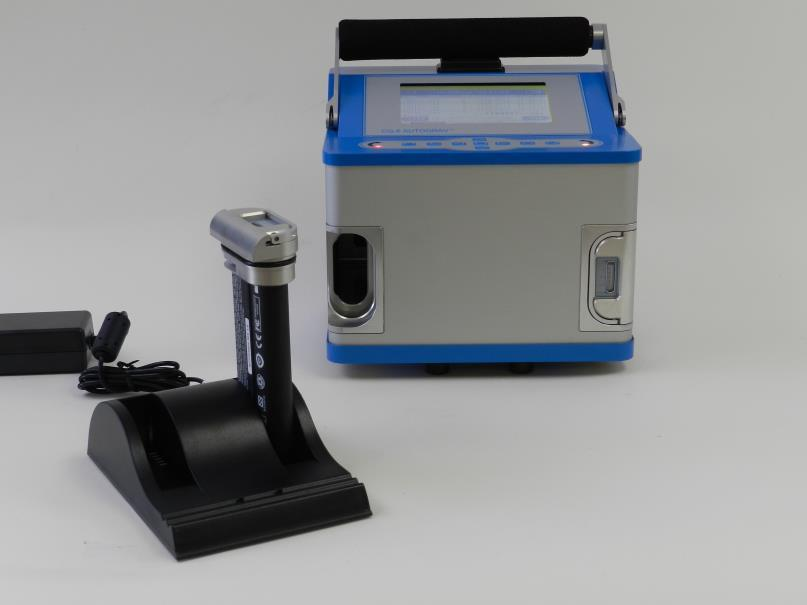
\includegraphics[width=0.7\textwidth]{figures/the_cg6_autograv_gravity_meter_and_the_battery_charger}
  \caption{\cg{} и устройство зарядки аккумуляторных батарей}
  \label{fig:the_cg6_autograv_gravity_meter_and_the_battery_charger}
\end{figure}

\section{Обзор главного экрана изображения}

\begin{figure}[h]
  \centering
  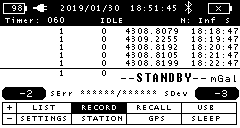
\includegraphics[width=0.49\textwidth]{figures/cg6_autograv_main_screen_idle_mode}
  \caption{Главный экран \cg{}: режим ожидания}
  \label{fig:cg6_autograv_main_screen_idle_mode}
\end{figure}

\begin{figure}[h]
  \centering
  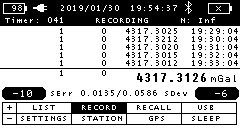
\includegraphics[width=0.49\textwidth]{figures/cg6_autograv_main_screen_recording_mode}
  \caption{Главный экран \cg{}: режим записи}
  \label{fig:cg6_autograv_main_screen_recording_mode}
\end{figure}

В верхней части главного экрана находятся; значки статуса батарей (с указанием
процента заряда каждой аккумуляторной батареи). Дата и время, показания таймера
(оставшееся время измерения текущего цикла в секундах, обратный отсчёт времени
регистрации), статус измерительного прибора (находится ли он в режиме
бездействия (IDLE) или в режиме регистрации данных (RECORDING)) и число циклов,
запрограммированное для проведения измерений.

\begin{figure}[h]
  \centering
  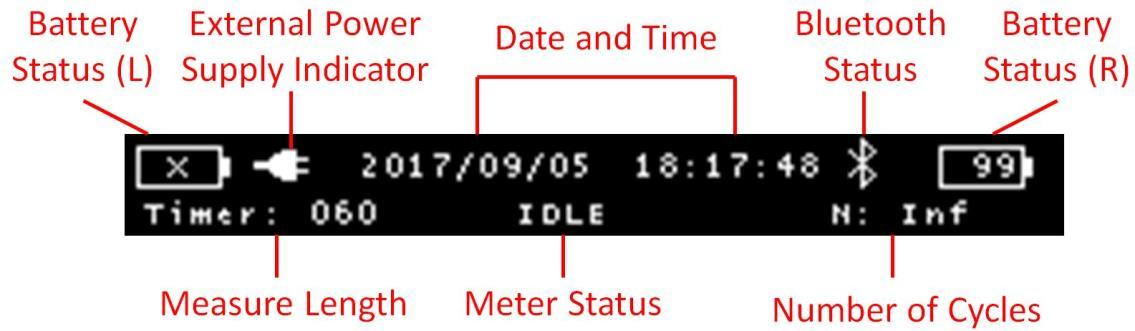
\includegraphics[width=0.7\textwidth]{figures/main_screen_upper_part}
  \caption{Главный экран: верхняя часть}
  \label{fig:main_screen_upper_part}
\end{figure}

В средней части экранного изображения отображаются предыдущие измерения силы
тяжести, где наиболее удалённые по времени измерения располагаются вверху
списка. Здесь отображаются также название пункта наблюдения, номер профиля,
величина измерения и время в конце взятия отсчётов. Эти измерения уже сохранены
в памяти прибора.

\begin{figure}[h]
  \centering
  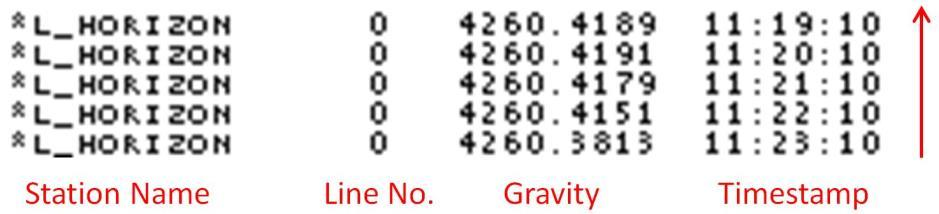
\includegraphics[width=0.7\textwidth]{figures/main_screen_middle_part}
  \caption{Главный экран: средняя часть}
  \label{fig:main_screen_middle_part}
\end{figure}

Под сплошной горизонтальной линией отображается: текущий пункт наблюдения и его
порядковый номер в списке пунктов наблюдения, номер профиля. А под ними –
величина измерения в мГал, величина стандартного отклонения (SDev) для отсчётов,
использованных для расчёта измерения, и величина стандартной ошибки (SErr,
равной стандартному отклонению, разделённому на квадратный корень из числа
текущих отсчётов $ SErr = SDev/\sqrt{N} $). Когда измеритель находится в режиме
ожидания, значение силы тяжести заменяется на <<STANDBY>> и значения SErr и SDev
будут *****

Слева показана величина наклона по оси X в арксекундах, а справа – величина
наклона по оси Y в арксекундах.

\begin{figure}[h]
  \centering
  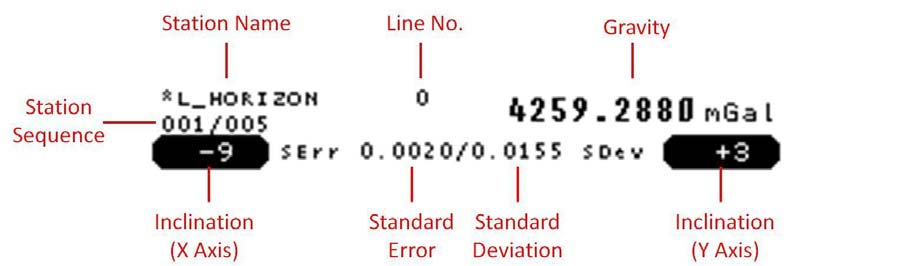
\includegraphics[width=0.7\textwidth]{figures/main_screen_lower_part}
  \caption{Главный экран: нижняя часть}
  \label{fig:main_screen_lower_part}
\end{figure}

В нижней части экрана располагаются наиболее часто используемые элементы меню.

\begin{figure}[h]
  \centering
  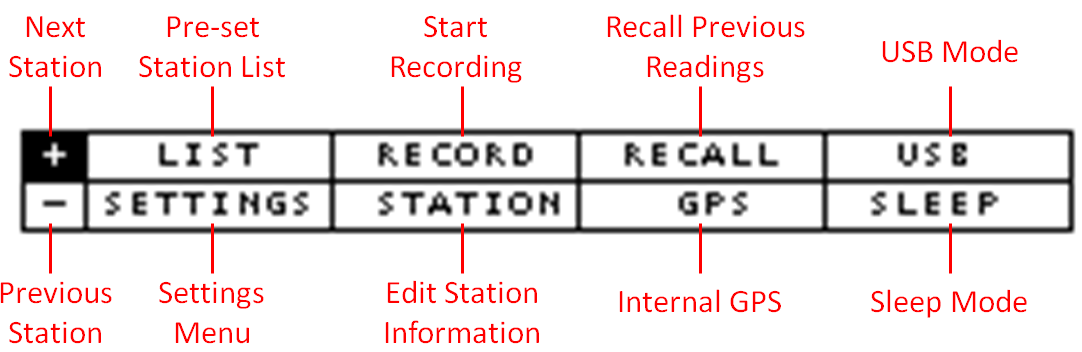
\includegraphics[width=0.7\textwidth]{figures/main_screen_menu}
  \caption{Меню главного экрана}
  \label{fig:main_screen_menu}
\end{figure}

\section{Базовые операции}

\subsection{Перемещение по меню}

При помощи кнопок управления осуществляется перемещение курсора.  Подтверждение
выбора или вход в подменю производится с помощью кнопки \textbf{Enter}.

\begin{figure}[h]
  \centering
  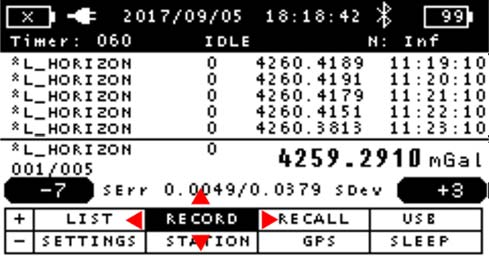
\includegraphics[width=0.49\textwidth]{figures/navigation_the_menus_1}
  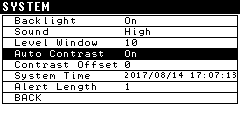
\includegraphics[width=0.49\textwidth]{figures/navigation_the_menus_2}
  \caption{Перемещение по меню}
  \label{fig:navigation_the_menus}
\end{figure}

\subsection{Снятие показаний}

Счётчик имеет два режима работы:
\begin{description}
  \item[RECORDING (ЗАПИСЬ):] Используется для записи измерений. В этом режиме
    отфильтрованное значение силы тяжести отображается на главном экране, как
    показано на рисунке~\ref{fig:cg6_autograv_main_screen_recording_mode}.

  \item[IDLE (ХОЛОСТОЙ ХОД):] Используется при перемещении прибора. Это
    сокращает время установки на следующей станции за счёт стабилизации
    электроники во время транспортировки. В этом режиме значение силы тяжести
    заменяется словом “STANDBY” на главном экране, как показано на
    рисунке~\ref{fig:cg6_autograv_main_screen_idle_mode}. 
\end{description}

Для переключения режима работы между \textit{\textbf{RECORDING}} и
\textit{\textbf{IDLE}}: поместите курсор на \textbf{RECORD} на главном экране и
нажмите кнопку \textbf{Enter}.

\subsection{Редактирование значений переменных}

\subsubsection{Как выделить значение в выбираемом списке}

\begin{figure}[h]
  \centering
  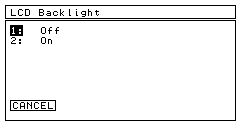
\includegraphics[width=0.49\textwidth]{figures/choosing_a_value_from_a_selectable_list}
  \caption{Выделение значения в выбираемом списке}
  \label{fig:choosing_a_value_from_a_selectable_list}
\end{figure}

Для того, чтобы выделить значение в выбираемом списке, достаточно навести курсор
на нужную запись и нажать кнопку \textbf{Enter}.

Чтобы покинуть это экранное изображение без изменений:
\begin{itemize}
  \item наведите курсор на пункт \textbf{CANCEL}, после чего нажмите кнопку
    \textbf{Enter}, или
  \item нажмите кнопку \textbf{Back}
\end{itemize}

\subsubsection{Ввод значения с экранной клавиатуры}
\label{subsubsec:entering_a_value_with_onscreen_keypad}

Некоторые переменные требуют редактирования с помощью экранной клавиатуры.  В
зависимости от типа переменной, экранная клавиатура может быть цифровой или
буквенно-цифровой.

\begin{figure}[h]
  \centering
  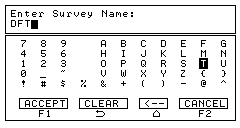
\includegraphics[width=0.49\textwidth]{figures/onscreen_keypad_numeric_and_alphanumeric_1}
  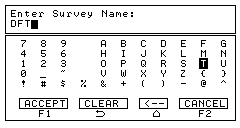
\includegraphics[width=0.49\textwidth]{figures/onscreen_keypad_numeric_and_alphanumeric_2}
  \caption{Экранная клавиатура: цифровая и буквенно-цифровая}
  \label{fig:onscreen_keypad_numeric_and_alphanumeric}
\end{figure}

Чтобы ввести символ в поле, переместите курсор на нужный символ и нажмите кнопку
\textbf{Enter}.

Чтобы стереть последний символ в поле, переместите курсор на $\leftarrow$ , используя:
\begin{itemize}
  \item кнопки навигации \textbf{Navigation}, или
  \item кнопку \textbf{Home}
\end{itemize}
и нажмите кнопку \textbf{Enter}.

Чтобы очистить все поле, переместите курсор на \textbf{<<CLEAR>>} используя:
\begin{itemize}
  \item кнопки навигации \textbf{Navigation}, или
  \item кнопку \textbf{Back}
\end{itemize}
и нажмите кнопку \textbf{Enter}.

Чтобы принять значение в поле, переместите курсор на \textbf{<<ACCEPT>>} используя:
\begin{itemize}
  \item кнопки навигации \textbf{Navigation}, или
  \item кнопку \textbf{F1}
\end{itemize}
и нажмите кнопку \textbf{Enter}.

Чтобы выйти из этого экрана без изменений, переместите курсор на
\textbf{<<CANCEL>>}, используя:
\begin{itemize}
  \item кнопки навигации \textbf{Navigation}, или
  \item кнопку \textbf{F2}
\end{itemize}
и нажмите кнопку \textbf{Enter}.

\section[Спящий режим]{Ввод/вывод прибора \cg{} в/из спящего режима}

Прибор \cg{} может быть переведён в спящий режим, когда бездействует главный
дисплей и стрелки выравнивания. Однако, сам прибор остаётся в рабочем состоянии.

\begin{figure}[h]
  \centering
  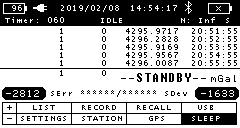
\includegraphics[width=0.49\textwidth]{figures/the_main_screen_ready_for_sleep_mode}
  \caption{Главный экран готов к спящему режиму}
  \label{fig:the_main_screen_ready_for_sleep_mode}
\end{figure}

На главном экранном изображении при помощи \textbf{кнопок управления Navigation}
наведите курсор на пункт \textbf{SLEEP} и нажмите кнопку \textbf{Enter}.

\infobox{
  Когда прибор \cg{} находится в спящем режиме, нажатие любой кнопки приведёт к
  его <<пробуждению>>.
}

\chapter[Настройка]{Настройка \cg{}}
\label{chap:setting_up_your_cg6_autograv}

Гравиметр \cg{} имеет дополнительный планшетный компьютер (номер по каталогу
888030), который позволяет пользователю быстро настроить и спланировать съёмку с
помощью предварительно загруженного программного обеспечения LynxLG.
Пожалуйста, обратитесь к Руководству по программному обеспечению LynxLG
Acquisition (p/n 115370003) для получения дополнительной информации о настройке
с помощью планшетного компьютера.

\infobox{
  Вы можете управлять работой прибора \cg{} как с помощью планшетного компьютера
  (\textnumero{} 888030), так и без него. Прибор \cg{} снабжён программным
  обеспечением и пользовательским интерфейсом, который позволяет пользоваться
  прибором как полнофункциональным автономным гравиметром. Режим планшетного
  компьютера предоставляет вам больше возможностей и позволяет дистанционно
  управлять работой прибора \cg{}. Кроме того, в этом режиме пользователю
  предоставляется доступ к расширенным функциональным возможностям, таким,
  например, как создание координатных карт пунктов наблюдения для определения
  местоположения в реальном времени, средства импорта пунктов
  наблюдения/маршрута (KML, GPX, Delimited ASCII), и создание простых карт
  редукций Буге.
}

\section{Меню настроек Settings}

На главном экранном изображении наведите курсор на пункт \textbf{SETTINGS}
(изображение внизу слева) и нажмите кнопку \textbf{Enter}. Откроется экран,
показанный справа:

\begin{figure}[H]
  \centering
  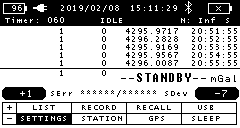
\includegraphics[width=0.49\textwidth]{figures/the_settings_screen_1}
  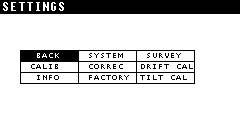
\includegraphics[width=0.49\textwidth]{figures/the_settings_screen_2}
  \caption{Экран меню настроек}
  \label{fig:the_settings_screen}
\end{figure}

\section{Настройка системы}

Чтобы получить доступ к экранному изображению настроек системы, наведите курсор
на пункт \textbf{SYSTEM} (изображение внизу слева) и нажмите кнопку
\textbf{Enter}.  Откроется экран, показанный справа:

\begin{figure}[H]
  \centering
  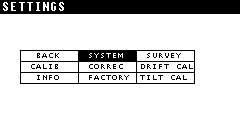
\includegraphics[width=0.49\textwidth]{figures/the_system_screen_1}
  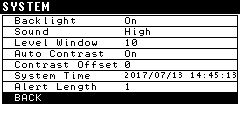
\includegraphics[width=0.49\textwidth]{figures/the_system_screen_2}
  \caption{Экран системы}
  \label{fig:the_system_screen}
\end{figure}

\subsection{Включение и выключение фоновой подсветки экрана}

Фоновая подсветка экрана может находиться в одном из двух состояний: ON или OFF.
Для настройки фоновой подсветки наведите курсор на пункт \textbf{Backlight}
(изображение внизу слева) и нажмите кнопку \textbf{Enter}. Откроется экран,
показанный справа:

\newpage
\begin{figure}[H]
  \centering
  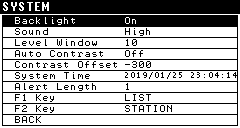
\includegraphics[width=0.49\textwidth]{figures/the_backlight_screen_1}
  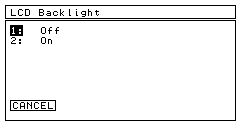
\includegraphics[width=0.49\textwidth]{figures/the_backlight_screen_2}
  \caption{Экран настройки фоновой подсветки}
  \label{fig:the_backlight_screen}
\end{figure}

Фоновую подсветку можно включить (\textbf{On}) или выключить (\textbf{Off}).
Наведите курсор на символ 1 или 2 и нажмите кнопку \textbf{Enter}.

Чтобы покинуть это экранное изображение без изменений:
\begin{itemize}
  \item наведите курсор на пункт \textbf{CANCEL}, после чего нажмите кнопку
    \textbf{Enter}, или

  \item нажмите кнопку \textbf{Back}
\end{itemize}

\subsection{Настройка громкости звукового сигнала}

Для громкости звукового сигнала предусмотрено четыре варианта выбора: Low
(Низкая), Medium (Средняя), High (Высокая) или Disabled (Отключена). Для
настройки громкости наведите курсор на пункт \textbf{Sound} (изображение внизу
слева) и нажмите кнопку \textbf{Enter}. Откроется экран, показанный справа:

\begin{figure}[H]
  \centering
  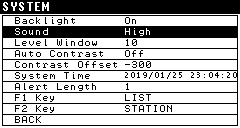
\includegraphics[width=0.49\textwidth]{figures/the_buzzer_volume_screen_1}
  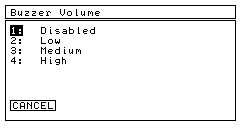
\includegraphics[width=0.49\textwidth]{figures/the_buzzer_volume_screen_2}
  \caption{Экран настройки громкости звукового сигнала}
  \label{fig:the_buzzer_volume_screen}
\end{figure}

Наведите курсор на пункт, соответствующий нужной громкости, и нажмите кнопку
\textbf{Enter}.

Чтобы покинуть это экранное изображение без изменений:
\begin{itemize}
  \item наведите курсор на пункт \textbf{CANCEL}, после чего нажмите кнопку
    \textbf{Enter}, или

  \item нажмите кнопку \textbf{Back}
\end{itemize}

\subsection{Регулировка окна горизонтирования}
\label{subsec:adjusting_the_level_window}

\infobox{
  Величина окна горизонтирования~-- это порог, ниже которого цвет стрелок
  горизонтирования становится зелёным.  Например, если интервал горизонтирования задан
  равным 10 угловых секунд, тогда в случае, когда величина угла наклона одной из
  осей не выходит за пределы \textpm{}10 угловых секунд, соответствующая этой
  оси стрелка горизонтирования имеет зелёный цвет.
}

Для корректировки величины окна горизонтирования наведите курсор на пункт
\textbf{Level} \textbf{Window} (изображение внизу слева) и нажмите кнопку
\textbf{Enter}. Откроется экран, показанный справа:

\begin{figure}[H]
  \centering
  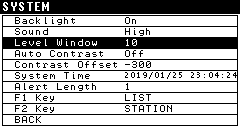
\includegraphics[width=0.49\textwidth]{figures/the_level_window_size_editing_screen_1}
  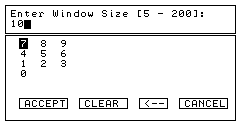
\includegraphics[width=0.49\textwidth]{figures/the_level_window_size_editing_screen_2}
  \caption{Экран выбора величины окна горизонтирования}
  \label{fig:the_level_window_size_editing_screen}
\end{figure}

Введите желаемый размер окна с помощью экранной клавиатуры, как описано в
разделе \nameref{subsubsec:entering_a_value_with_onscreen_keypad}.

\subsection{Включение/выключение автоматического изменения контрастности}

Функция автоматического изменения контрастности экранного изображения может
находиться в одном из двух состояний~-- ON или OFF. В общем случае, функция
автоматического изменения контрастности всегда должна быть включена. Тогда
регулирование контрастности будет осуществляться автоматически с учётом
температуры ЖК-дисплея. Это удобно при работе в поле, когда количество
солнечного света и внешняя температура могут сильно меняться в течение дня.
Чтобы включить или выключить функцию автоматического изменения контрастности
наведите курсор на пункт \textbf{Auto Contrast} (изображение внизу слева) и
нажмите кнопку \textbf{Enter}. Откроется экран, показанный справа:

\begin{figure}[H]
  \centering
  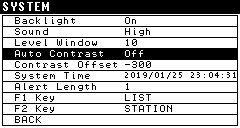
\includegraphics[width=0.49\textwidth]{figures/the_auto_contrast_screen_1}
  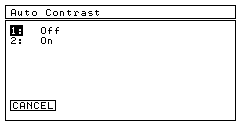
\includegraphics[width=0.49\textwidth]{figures/the_auto_contrast_screen_2}
  \caption{Экран функции автоматического изменения контрастности}
  \label{fig:the_auto_contrast_screen}
\end{figure}

Чтобы включить (\textbf{On}) или выключить (\textbf{Off}) функцию
автоматического изменения контрастности, наведите курсор на символ 1 или 2 и
нажмите кнопку \textbf{Enter}.

Чтобы покинуть это экранное изображение без изменений:
\begin{itemize}
  \item наведите курсор на пункт \textbf{CANCEL}, после чего нажмите кнопку
    \textbf{Enter}, или

  \item нажмите кнопку \textbf{Back}
\end{itemize}

\infobox{
  В общем случае, функция автоматического изменения контрастности всегда должна
  быть включена. Тогда регулирование контрастности будет осуществляться
  автоматически с учётом температуры ЖК-дисплея.
}

\subsection{Регулировка смещения контрастности экрана}

Помимо автоматической регулировки контрастности экранного изображения (см.
предыдущий раздел) вы также можете корректировать смещение контрастности (т.~е.,
яркость). Чем выше будет значение, тем темнее будет экранное изображение.  Для
редактирования величины смещения контрастности, наведите курсор на пункт
\textbf{Contrast Offset} (изображение внизу слева) и нажмите кнопку
\textbf{Enter}. Откроется экран, показанный справа:

\begin{figure}[H]
  \centering
  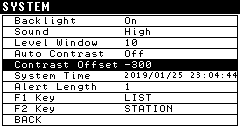
\includegraphics[width=0.49\textwidth]{figures/the_contrast_offset_editing_screen_1}
  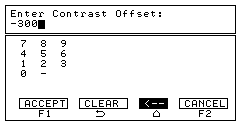
\includegraphics[width=0.49\textwidth]{figures/the_contrast_offset_editing_screen_2}
  \caption{Экран редактирования смещения контрастности}
  \label{fig:the_contrast_offset_editing_screen}
\end{figure}

Смещение контрастности может быть установлено на любое значение от -500 до
+1000.

Введите желаемое смещение контрастности с экранной клавиатуры, как описано в
разделе \nameref{subsubsec:entering_a_value_with_onscreen_keypad}

\infobox{
  Чем больше вводимая величина смещения контрастности, тем темнее будет ваше
  экранное изображение.
}

\subsection{Корректировка системных даты и времени}

\infobox{
  Вы можете ввести системные дату и время вручную, или синхронизировать их по
  GPS.
}

\subsubsection{Как ввести системные дату и время вручную}

Для корректировки системного времени, наведите курсор на пункт \textbf{System
  Time} (изображение внизу слева) и нажмите кнопку \textbf{Enter}. Откроется
экран, показанный справа:

\newpage
\begin{figure}[H]
  \centering
  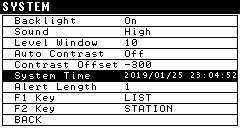
\includegraphics[width=0.49\textwidth]{figures/the_system_time_editing_screen_1}
  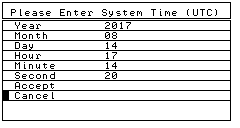
\includegraphics[width=0.49\textwidth]{figures/the_system_time_editing_screen_2}
  \caption{Экран редактирования системного времени}
  \label{fig:the_system_time_editing_screen_1}
\end{figure}

Чтобы ввести год, наведите курсор на пункт \textbf{Year} (год, изображение внизу
слева) и нажмите кнопку \textbf{Enter}. Откроется экран, показанный справа:

\begin{figure}[H]
  \centering
  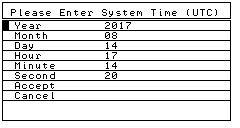
\includegraphics[width=0.49\textwidth]{figures/the_system_time_editing_screen_3}
  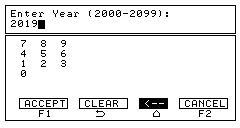
\includegraphics[width=0.49\textwidth]{figures/the_system_time_editing_screen_4}
  \caption{Экран редактирования системного времени}
  \label{fig:the_system_time_editing_screen_2}
\end{figure}

Введите значение года с помощью клавиатуры на экранной клавиатуре, как
описано в разделе \nameref{subsubsec:entering_a_value_with_onscreen_keypad}.

Повторите ту же процедуру для настройки месяца (month), дня (day), часа (hour),
минуты (minute) и секунды (second).

Чтобы принять новое значение системного времени, переместите курсор на
\textbf{Accept}
(на экране слева на рисунке~\ref{fig:the_system_time_editing_screen_2}) и
нажмите кнопку \textbf{Enter}.

\subsubsection{Обновление системных даты и времени при помощи встроенного блока
  GPS}

На главном экранном изображении наведите курсор на пункт \textbf{GPS} (изображение
внизу слева) и нажмите кнопку \textbf{Enter}. Откроется экран, показанный справа:

\begin{figure}[H]
  \centering
  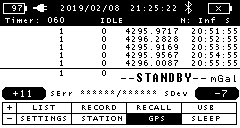
\includegraphics[width=0.49\textwidth]{figures/the_gps_screen_1}
  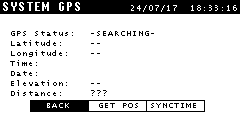
\includegraphics[width=0.49\textwidth]{figures/the_gps_screen_2}
  \caption{Экран GPS}
  \label{fig:the_gps_screen_1}
\end{figure}

\infobox{
  Поначалу статус блока GPS будет определён как <<SEARCHING>> (В процессе
  поиска).  Чтобы улучшить качество приёма сигнала, поместите прибор \cg{} в такое
  место, где он будет находиться под открытым небом.
}

После установления соединения статус блока GPS поменяется на <<LOCKED>> (Сигнал
захвачен). Поля Latitude (Широта), Longitude (Долгота), Time (Время), Date
(Дата), Elevation (Высота над у/моря) и Distance (Расстояние) будут заполнены
автоматически.

Наведите курсор на ячейку \textbf{SYNCTIME} и нажмите кнопку \textbf{Enter}. В
результате системное время будет синхронизировано со встроенным блоком GPS.

\begin{figure}[H]
  \centering
  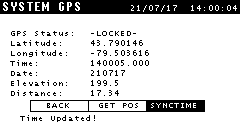
\includegraphics[width=0.49\textwidth]{figures/gps_time_synced}
  \caption{Синхронизированное время GPS}
  \label{fig:gps_time_synced}
\end{figure}

\subsection{Настройка длительности оповещения}

Длительность оповещения (в секундах)~-- это период времени, в течение которого
стрелки горизонтирования мигают красным цветом, свидетельствуя о том, что измерение
выполнено. Для редактирования длительности оповещения, наведите курсор на пункт
\textbf{Alert Length} (изображение внизу слева) и нажмите кнопку \textbf{Enter}.
Откроется экран, показанный справа:

\begin{figure}[H]
  \centering
  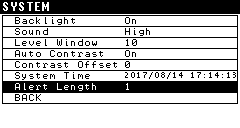
\includegraphics[width=0.49\textwidth]{figures/the_alert_length_editing_screen_1}
  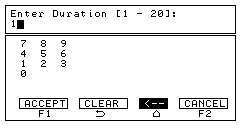
\includegraphics[width=0.49\textwidth]{figures/the_alert_length_editing_screen_2}
  \caption{Экран редактирования длительности оповещения}
  \label{fig:the_alert_length_editing_screen}
\end{figure}

Длительность оповещения может принимать любое значение в интервале от 1 секунды
до 20 секунд.

Введите желаемое значение задержки длины предупреждения с помощью экранной
клавиатуры, как описано в разделе
\nameref{subsubsec:entering_a_value_with_onscreen_keypad}.

\subsection{Назначение функций для кнопок F1 и F2}

Пользовательские функции для пунктов меню главного экрана могут быть назначены
пользователем кнопкам F1 и F2.

Чтобы назначить функцию кнопке \textbf{F1}, переместите курсор на клавишу
\textbf{F1} (изображение внизу слева) и нажмите кнопку \textbf{Enter}. Появится
экран справа:

Переместите курсор на желаемую функцию для быстрого доступа и нажмите
кнопку \textbf{Enter}.

Чтобы покинуть это экранное изображение без изменений:
\begin{itemize}
  \item наведите курсор на пункт \textbf{CANCEL}, после чего нажмите кнопку
    \textbf{Enter}, или

  \item нажмите кнопку \textbf{Back}.
\end{itemize}

\begin{figure}[H]
  \centering
  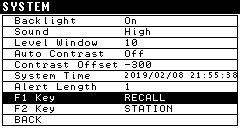
\includegraphics[width=0.49\textwidth]{figures/assigning_a_shortcut_to_the_f1_button_1}
  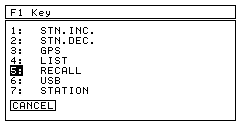
\includegraphics[width=0.49\textwidth]{figures/assigning_a_shortcut_to_the_f1_button_2}
  \caption{Назначение функции кнопке F1}
  \label{fig:assigning_a_shortcut_to_the_f1_button}
\end{figure}

Выполните ту же процедуру, чтобы назначить функцию кнопке F2.

\section{Настройки параметров съёмки}

Чтобы получить доступ к экранному изображению настройки параметров съёмки,
наведите курсор на пункт \textbf{SURVEY} (изображение внизу слева) и нажмите кнопку
\textbf{Enter}. Откроется экран, показанный справа:

\begin{figure}[H]
  \centering
  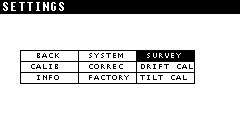
\includegraphics[width=0.49\textwidth]{figures/the_survey_setting_screen_1}
  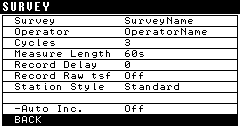
\includegraphics[width=0.49\textwidth]{figures/the_survey_setting_screen_2}
  \caption{Экран настройки параметров съёмки}
  \label{fig:the_survey_setting_screen}
\end{figure}

\subsection{Редактирование названия съёмки}

Чтобы изменить название съёмки, наведите курсор на пункт \textbf{Survey}
(изображение внизу слева) и нажмите кнопку \textbf{Enter}. Откроется экран,
показанный справа:

\newpage
\begin{figure}[H]
  \centering
  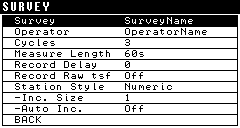
\includegraphics[width=0.49\textwidth]{figures/the_survey_name_editing_screen_1}
  \includegraphics[width=0.49\textwidth]{figures/the_survey_name_editing_screen_2}
  \caption{Экран редактирования названия съёмки}
  \label{fig:the_survey_name_editing_screen}
\end{figure}

Название съёмки может представлять собой ту или иную комбинацию
буквенно-цифровых символов числом до 31.

Введите желаемое название съёмки с помощью экранной клавиатуры, как описано
в разделе \nameref{subsubsec:entering_a_value_with_onscreen_keypad}.

\subsection{Редактирование имени оператора}

Чтобы изменить имя оператора, наведите курсор на пункт \textbf{Operator}
(изображение внизу слева) и нажмите кнопку \textbf{Enter}. Откроется экран,
показанный справа:

\begin{figure}[H]
  \centering
  \includegraphics[width=0.49\textwidth]{figures/the_operator_name_editing_screen_1}
  \includegraphics[width=0.49\textwidth]{figures/the_operator_name_editing_screen_2}
  \caption{Экран редактирования имени оператора}
  \label{fig:the_operator_name_editing_screen}
\end{figure}

Имя оператора может представлять собой комбинацию буквенно-цифровых
символов числом до 31 знака.

Введите желаемое имя оператора с экранной клавиатуры, как описано в разделе
\nameref{subsubsec:entering_a_value_with_onscreen_keypad}.

\subsection{Настройка числа циклов}
\label{subsec:adjusting_the_number_of_cycles}

Для настройки числа циклов измерения на вашем пункте наблюдения наведите курсор
на строку \textbf{Cycles} (изображение внизу слева) и нажмите кнопку
\textbf{Enter}.  Откроется экран, показанный справа:

\begin{figure}[H]
  \centering
  \includegraphics[width=0.49\textwidth]{figures/the_cycles_screen_1}
  \includegraphics[width=0.49\textwidth]{figures/the_cycles_screen_2}
  \caption{Экран циклов}
  \label{fig:the_cycles_screen}
\end{figure}

\infobox{
  Число циклов определяется как количество успешных повторений отсчётов прибора
  на данном пункте наблюдения. Этот параметр может принимать любое значение в
  интервале от 1 до бесконечности, по вашему выбору. Число циклов, равное 0,
  соответствует бесконечности. Это значит, что гравиметр переведён в режим
  циклической работы, и будет выполнять измерения до тех пор, пока процесс
  снятия показаний не будет остановлен оператором.
}

Введите желаемое количество циклов с помощью экранной клавиатуры, как
описано в разделе \nameref{subsubsec:entering_a_value_with_onscreen_keypad}.

\subsection{Выбор длительности цикла измерения}
\label{subsec:adjusting_the_measurement_cycle_length}

Чтобы задать длительность одного измерения, наведите курсор на пункт
\textbf{Measure Length} (изображение внизу слева) и нажмите кнопку
\textbf{Enter}. Откроется экран, показанный справа:

\newpage
\begin{figure}[H]
  \centering
  \includegraphics[width=0.49\textwidth]{figures/the_measure_length_screen_1}
  \includegraphics[width=0.49\textwidth]{figures/the_measure_length_screen_2}
  \caption{Экран выбора длительности измерения}
  \label{fig:the_measure_length_screen}
\end{figure}

Длительность измерения можно задать равной 15 секундам, 30 секундам, 60 секундам
или 120 секундам. Наведите курсор на нужное значение и нажмите кнопку
\textbf{Enter}.

Чтобы покинуть это экранное изображение без изменений:
\begin{itemize}
  \item наведите курсор на пункт \textbf{CANCEL}, после чего нажмите кнопку
    \textbf{Enter}, или

  \item нажмите кнопку \textbf{Back}.
\end{itemize}

\subsection{Корректировка задержки записи}

Вы можете ввести величину задержки записи в секундах~-- начало регистрации
данных будет отложено на это время. Это удобно при работе в поле, или во время
проверки калибровки дрейфа, когда вы хотите отложить начало снятия измерений.

Для редактирования величины задержки записи, наведите курсор на пункт
\textbf{Record Delay} (изображение внизу слева) и нажмите кнопку \textbf{Enter}.
Откроется экран, показанный справа:

\begin{figure}[H]
  \centering
  \includegraphics[width=0.49\textwidth]{figures/the_record_delay_editing_screen_1}
  \includegraphics[width=0.49\textwidth]{figures/the_record_delay_editing_screen_2}
  \caption{Экран редактирования задержки записи}
  \label{fig:the_record_delay_editing_screen}
\end{figure}

Задержка записи может принимать любое значение от 0 до бесконечности, по
вашему выбору.

Введите значение задержки записи с экранной клавиатуры, как описано в разделе
\nameref{subsubsec:entering_a_value_with_onscreen_keypad}.

\subsection{Активизация/отключение функции записи файла исходных данных TSF}

У вас есть возможность активизировать или отключить функцию записи файла
исходных данных .tsf (в дополнение к файлу фильтрованных данных .dat, который
записывается всегда).

Наведите курсор на пункт \textbf{Record Raw tsf} и нажмите кнопку
\textbf{Enter}. На дисплее появится следующее экранное изображение:

Чтобы активизировать (on) или отключить (off) функцию записи файла исходных
данных .tsf, наведите курсор на пункт \textbf{Record Raw tsf} (изображение внизу
слева) и нажмите кнопку \textbf{Enter}. Откроется экран, показанный справа:

\begin{figure}[H]
  \centering
  \includegraphics[width=0.49\textwidth]{figures/the_tsf_recording_screen_1}
  \includegraphics[width=0.49\textwidth]{figures/the_tsf_recording_screen_2}
  \caption{Экран записи файла tsf}
  \label{fig:the_tsf_recording_screen}
\end{figure}

Наведите курсор на символ 1 или 2 и нажмите кнопку \textbf{Enter}.

Чтобы покинуть это экранное изображение без изменений:
\begin{itemize}
  \item наведите курсор на пункт \textbf{CANCEL}, после чего нажмите кнопку
    \textbf{Enter}, или

  \item нажмите кнопку \textbf{Back}.
\end{itemize}

\subsection{Изменение стиля представления пункта наблюдения}

Для того, чтобы изменить стиль представления пункта наблюдения, наведите курсор
на пункт \textbf{Station Style} (изображение внизу слева) и нажмите кнопку
\textbf{Enter}.

Откроется экран, показанный справа:

\begin{figure}[H]
  \centering
  \includegraphics[width=0.49\textwidth]{figures/the_station_style_editing_screen_1}
  \includegraphics[width=0.49\textwidth]{figures/the_station_style_editing_screen_2}
  \caption{Экран редактирования стиля пункта наблюдения}
  \label{fig:the_station_style_editing_screen}
\end{figure}

Стиль представления пункта наблюдения может быть стандартным
(\textbf{Standard}), т.~е., представлять собой любое буквенно-цифровое
наименование, или цифровым (\textbf{Numeric}). Наведите курсор на символ 1 или 2
и нажмите кнопку \textbf{Enter}.

В зависимости от выбранного вами стиля представления пункта наблюдения, меню
съёмки будет немного отличаться, как показано на рисунке внизу.

\begin{figure}[H]
  \centering
  \includegraphics[width=0.49\textwidth]{figures/station_style_standard_vs_numeric_1}
  \includegraphics[width=0.49\textwidth]{figures/station_style_standard_vs_numeric_2}
  \caption{Стили представления пункта наблюдения: Standard и Numeric}
  \label{fig:station_style_standard_vs_numeric}
\end{figure}

Как можно заметить, параметр <<Inc. Size>> появляется только, когда выбран
цифровой стиль представления пункта наблюдения.

\subsection{Выбор шага приращения (только для цифрового стиля)}

Чтобы изменить величину шага приращения, наведите курсор на пункт \textbf{-Inc.
  Size} (изображение внизу слева) и нажмите кнопку \textbf{Enter}. Откроется
экран, показанный справа:

\begin{figure}[H]
  \centering
  \includegraphics[width=0.49\textwidth]{figures/the_increment_size_screen_1}
  \includegraphics[width=0.49\textwidth]{figures/the_increment_size_screen_2}
  \caption{Экран выбора шага приращения}
  \label{fig:the_increment_size_screen}
\end{figure}

Введите размер приращения с экранной клавиатуры, как описано в разделе
\nameref{subsubsec:entering_a_value_with_onscreen_keypad}.

Чтобы покинуть это экранное изображение без изменений:
\begin{itemize}
  \item наведите курсор на пункт \textbf{CANCEL}, после чего нажмите кнопку
    \textbf{Enter}, или

  \item нажмите кнопку \textbf{Back}.
\end{itemize}

\subsection{Активация/отключение автоматического перехода к следующему пункту}

Функция \textbf{Auto station increment} автоматически переводит ваш прибор CG-6
к следующему пункту наблюдения после выполнения всех циклов измерения на текущем
пункте наблюдения.

В числовом стиле станции новое имя станции будет представлять собой значение
текущей станции плюс размер приращения.

В стандартном стиле станции имя новой станции будет следующей станцией в
предварительно установленном списке станций. Широта, долгота, высота и номер
линии станции также будут обновлены соответственно.

Чтобы включить или отключить автоматическое приращение станции, переместите
курсор на \textbf{-Auto Inc} (изображение внизу слева) и нажмите кнопку
\textbf{Enter}. Появится экран справа:

\begin{figure}[H]
  \centering
  \includegraphics[width=0.49\textwidth]{figures/the_automatic_increment_screen_1}
  \includegraphics[width=0.49\textwidth]{figures/the_automatic_increment_screen_2}
  \caption{Экран функции автоматического перехода}
  \label{fig:the_automatic_increment_screen}
\end{figure}

Наведите курсор на символ 1 или 2 и нажмите кнопку \textbf{Enter}.

Чтобы покинуть это экранное изображение без изменений:
\begin{itemize}
  \item наведите курсор на пункт \textbf{CANCEL}, после чего нажмите кнопку
    \textbf{Enter}, или

  \item нажмите кнопку \textbf{Back}.
\end{itemize}

\section{Просмотр и изменение параметров калибровки}

На экранном изображении Settings наведите курсор на пункт \textbf{CALIB}
(изображение внизу слева) и нажмите кнопку \textbf{Enter}. Откроется экран,
показанный справа:

\begin{figure}[H]
  \centering
  \includegraphics[width=0.49\textwidth]{figures/the_instrument_parameter_screen_1}
  \includegraphics[width=0.49\textwidth]{figures/the_instrument_parameter_screen_2}
  \caption{Экран параметров прибора}
  \label{fig:the_instrument_parameter_screen}
\end{figure}

\newpage
\warningbox{
  Параметры прибора задаются на заводе-изготовителе Scintrex, и они
  индивидуальны для каждого гравиметра \cg{}:

  \begin{itemize}
    \item В обычных условиях оператор не должен изменять параметры
      \textbf{TEMP COEFF} и \textbf{TEMP SCALE}

    \item Параметр \textbf{GCAL1} может быть изменён только в случае повторной
      калибровки прибора \cg{}

    \item Параметр \textbf{DRIFT RATE} изменяется после проверки калибровки
      дрейфа

    \item Параметр \textbf{DRIFT START} может быть изменён в любое время, но
      обычно после проверки калибровки дрейфа

    \item Параметры \textbf{X SCALE}, \textbf{X OFFSET}, \textbf{Y SCALE},
      \textbf{Y OFFSET} изменяются после проверки калибровки дрейфа

    \item Параметр \textbf{G REF} может быть изменён в любое время в случае
      необходимости
  \end{itemize}
}

\subsection{Как изменить гравиметрическую постоянную GCAL1}

Чтобы изменить гравиметрическую постоянную \textbf{GCAL1}, наведите курсор на
пункт GCAL1 (изображение внизу слева) и нажмите кнопку \textbf{Enter}. Откроется
экран, показанный справа:

\begin{figure}[H]
  \centering
  \includegraphics[width=0.49\textwidth]{figures/the_gcal1_editing_screen_1}
  \includegraphics[width=0.49\textwidth]{figures/the_gcal1_editing_screen_2}
  \caption{Экран редактирования GCAL1}
  \label{fig:the_gcal1_editing_screen}
\end{figure}

Величина GCAL1 задаётся на заводе-изготовителе, и в обычных условиях изменять её
не следует.

Однако, если вы решите перекалибровать свой \cg{}, новое значение GCAL1 можно
будет ввести с экранной клавиатуры, как описано в разделе
\nameref{subsubsec:entering_a_value_with_onscreen_keypad}.

Чтобы покинуть это экранное изображение без изменений:
\begin{itemize}
  \item наведите курсор на пункт \textbf{CANCEL}, после чего нажмите кнопку
    \textbf{Enter}, или

  \item нажмите кнопку \textbf{Back}.
\end{itemize}

\subsection{Как изменить опорную величину силы тяжести}

Чтобы отредактировать опорную величину силы тяжести, наведите курсор на пункт
\textbf{G REF} (изображение внизу слева) и нажмите кнопку \textbf{Enter}.
Откроется экран, показанный справа:

\begin{figure}[H]
  \centering
  \includegraphics[width=0.49\textwidth]{figures/the_gravity_reference_value_editing_screen_1}
  \includegraphics[width=0.49\textwidth]{figures/the_gravity_reference_value_editing_screen_2}
  \caption{Экран редактирования опорной величины силы тяжести}
  \label{fig:the_gravity_reference_value_editing_screen}
\end{figure}

Опорная величина силы тяжести может принимать любое значение в диапазоне от 0 до
8000 мГал. Эта величина вычитается из текущего показания силы тяжести.

Введите новое значение величины опорной силы тяжести с помощью экранной
клавиатуры, как описано в разделе
\nameref{subsubsec:entering_a_value_with_onscreen_keypad}.

Чтобы покинуть это экранное изображение без изменений:
\begin{itemize}
  \item наведите курсор на пункт \textbf{CANCEL}, после чего нажмите кнопку
    \textbf{Enter}, или

  \item нажмите кнопку \textbf{Back}.
\end{itemize}

\subsection{Как изменить температурный коэффициент}

\warningbox{
  В обычных условиях оператор не должен изменять величину параметра \textbf{TEMP
    COEFF}.
}

Чтобы изменить величину температурного коэффициента, наведите курсор на пункт
\textbf{TEMP COEFF} (изображение внизу слева) и нажмите кнопку \textbf{Enter}.
Откроется экран, показанный справа:

\begin{figure}[H]
  \centering
  \includegraphics[width=0.49\textwidth]{figures/the_temperature_coefficient_editing_screen_1}
  \includegraphics[width=0.49\textwidth]{figures/the_temperature_coefficient_editing_screen_2}
  \caption{Экран редактирования температурного коэффициента}
  \label{fig:the_temperature_coefficient_editing_screen}
\end{figure}

Температурный коэффициент является отрицательной величиной в диапазоне от
\textminus{}0,1 до \textminus{}0,2.

Введите новый температурный коэффициент с помощью экранной клавиатуры, как
описано в разделе \nameref{subsubsec:entering_a_value_with_onscreen_keypad}.

Чтобы покинуть это экранное изображение без изменений:
\begin{itemize}
  \item наведите курсор на пункт \textbf{CANCEL}, после чего нажмите кнопку
    \textbf{Enter}, или

  \item нажмите кнопку \textbf{Back}.
\end{itemize}

\subsection{Как изменить коэффициент усиления по температуре (TEMP SCALE)}

\warningbox{
  В обычных условиях оператор не должен изменять величину параметра \textbf{TEMP
    SCALE}.
}

Чтобы изменить величину коэффициента усиления по температуре, наведите курсор на
пункт \textbf{TEMP SCALE} (изображение внизу слева) и нажмите кнопку
\textbf{Enter}.  Откроется экран, показанный справа:

\begin{figure}[H]
  \centering
  \includegraphics[width=0.49\textwidth]{figures/the_temperature_gain_editing_screen_1}
  \includegraphics[width=0.49\textwidth]{figures/the_temperature_gain_editing_screen_2}
  \caption{Экран редактирования коэффициента усиления по температуре}
  \label{fig:the_temperature_gain_editing_screen}
\end{figure}

Введите новое значение прироста температуры с помощью экранной клавиатуры,
как описано в разделе \nameref{subsubsec:entering_a_value_with_onscreen_keypad}.

Чтобы покинуть это экранное изображение без изменений:
\begin{itemize}
  \item наведите курсор на пункт \textbf{CANCEL}, после чего нажмите кнопку
    \textbf{Enter}, или

  \item нажмите кнопку \textbf{Back}.
\end{itemize}

\subsection{Как изменить постоянные датчика наклона}

\infobox{Обычно новые постоянные датчика наклона вводятся автоматически при
  проведении проверки калибровки уровня, как описывается далее в этой главе.
  Показанные ниже действия позволяют вам вручную изменить постоянные датчика
  наклона в случае необходимости.}

Постоянные датчика наклона включают в себя: X Scale, X Offset, Y Scale и Y Offset.

Чтобы редактировать эти постоянные, наведите курсор на соответствующее поле
(изображение внизу слева) и нажмите кнопку \textbf{Enter}. Откроется экран,
показанный справа:

\newpage
\begin{figure}[H]
  \centering
  \includegraphics[width=0.49\textwidth]{figures/the_x_level_scale_editing_screen_1}
  \includegraphics[width=0.49\textwidth]{figures/the_x_level_scale_editing_screen_2}
  \caption{Экран редактирования шкалы уровня по оси X}
  \label{fig:the_x_level_scale_editing_screen}
\end{figure}

\begin{figure}[H]
  \centering
  \includegraphics[width=0.49\textwidth]{figures/the_x_level_offset_editing_screen_1}
  \includegraphics[width=0.49\textwidth]{figures/the_x_level_offset_editing_screen_2}
  \caption{Экран редактирования смещения уровня по оси X}
  \label{fig:the_x_level_offset_editing_screen}
\end{figure}

\begin{figure}[H]
  \centering
  \includegraphics[width=0.49\textwidth]{figures/the_y_level_scale_editing_screen_1}
  \includegraphics[width=0.49\textwidth]{figures/the_y_level_scale_editing_screen_2}
  \caption{Экран редактирования шкалы уровня по оси Y}
  \label{fig:the_y_level_scale_editing_screen}
\end{figure}

\begin{figure}[H]
  \centering
  \includegraphics[width=0.49\textwidth]{figures/the_y_level_offset_editing_screen_1}
  \includegraphics[width=0.49\textwidth]{figures/the_y_level_offset_editing_screen_2}
  \caption{Экран редактирования смещения уровня по оси Y}
  \label{fig:the_y_level_offset_editing_screen}
\end{figure}

С помощью экранной клавиатуры введите новое значение, как описано в разделе
\nameref{subsubsec:entering_a_value_with_onscreen_keypad}.

Чтобы покинуть это экранное изображение без изменений:
\begin{itemize}
  \item наведите курсор на пункт \textbf{CANCEL}, после чего нажмите кнопку
    \textbf{Enter}, или

  \item нажмите кнопку \textbf{Back}.
\end{itemize}

\subsection{Как изменить величину дрейфа}

\warningbox{
  Изменение скорости дрейфа или времени начала дрейфа приведёт к изменению ваших
  данных.
}

\infobox{
  Обычно новое значение величины дрейфа вводится автоматически при проведении
  проверки калибровки дрейфа, как описывается далее в этой главе.  Показанные
  ниже действия позволяют вам вручную изменить скорость дрейфа в случае
  необходимости.
}

Для редактирования величины скорости дрейфа, наведите курсор на пункт
\textbf{DRIFT RATE} (изображение внизу слева) и нажмите кнопку Enter. Откроется
экран, показанный справа:

\newpage
\begin{figure}[H]
  \centering
  \includegraphics[width=0.49\textwidth]{figures/the_drift_rate_editing_screen_1}
  \includegraphics[width=0.49\textwidth]{figures/the_drift_rate_editing_screen_2}
  \caption{Экран редактирования величины дрейфа}
  \label{fig:the_drift_rate_editing_screen}
\end{figure}

Введите новую скорость дрейфа с экранной клавиатуры, как описано в
\nameref{subsubsec:entering_a_value_with_onscreen_keypad}.

Чтобы покинуть это экранное изображение без изменений:
\begin{itemize}
  \item наведите курсор на пункт \textbf{CANCEL}, после чего нажмите кнопку
    \textbf{Enter}, или

  \item нажмите кнопку \textbf{Back}.
\end{itemize}

\subsection{Как изменить время начала компенсации дрейфа}

Время начала компенсации дрейфа~-- это момент времени, начиная с которого
производится компенсация дрейфа вашего прибора \cg{}. Это может быть любая дата в
интервале от прошлого до настоящего.

Для редактирования времени начала компенсации дрейфа, наведите курсор на пункт
\textbf{DRIFT START} (изображение внизу слева) и нажмите кнопку \textbf{Enter}.
Откроется экран, показанный справа:

\infobox{
  Вы можете вручную синхронизировать время начала компенсации дрейфа по
  юлианскому времени, используя для этого планшетный компьютер. Эта процедура
  более подробно описана в руководстве по программному обеспечению LynxLG (p/n
  115370003).
}

Для редактирования времени начала компенсации дрейфа, наведите курсор на пункт
\textbf{DRIFT START} (изображение внизу слева) и нажмите кнопку \textbf{Enter}.
Откроется экран, показанный справа:

\begin{figure}[H]
  \centering
  \includegraphics[width=0.49\textwidth]{figures/the_drift_start_time_editing_screen_1}
  \includegraphics[width=0.49\textwidth]{figures/the_drift_start_time_editing_screen_2}
  \caption{Экран редактирования времени начала дрейфа}
  \label{fig:the_drift_start_time_editing_screen}
\end{figure}

Чтобы ввести год, наведите курсор на пункт \textbf{Year} (изображение внизу слева) и
нажмите кнопку \textbf{Enter}. Откроется экран, показанный справа:

\begin{figure}[H]
  \centering
  \includegraphics[width=0.49\textwidth]{figures/the_year_editing_screen_1}
  \includegraphics[width=0.49\textwidth]{figures/the_year_editing_screen_2}
  \caption{Экран редактирования года}
  \label{fig:the_year_editing_screen_1}
\end{figure}

Введите год с экранной клавиатуры, как описано в разделе
\nameref{subsubsec:entering_a_value_with_onscreen_keypad}.

Чтобы покинуть это экранное изображение без изменений:
\begin{itemize}
  \item наведите курсор на пункт \textbf{CANCEL}, после чего нажмите кнопку
    \textbf{Enter}, или

  \item нажмите кнопку \textbf{Back}.
\end{itemize}

Аналогичную процедуру нужно выполнить, чтобы отредактировать месяц, день, час,
минуты и секунды.

\section{Поправки к показаниям прибора}

В вашем приборе \cg{} вы можете активизировать или отключить функцию введения
поправок на температуру, дрейф, земные приливы или на наклон.

На экранном изображении Settings наведите курсор на пункт \textbf{CORREC}
(изображение внизу слева) и нажмите кнопку \textbf{Enter}. Откроется экран,
показанный справа:

\begin{figure}[H]
  \centering
  \includegraphics[width=0.49\textwidth]{figures/the_instrument_corrections_screen_1}
  \includegraphics[width=0.49\textwidth]{figures/the_instrument_corrections_screen_2}
  \caption{Экран поправок к показаниям прибора}
  \label{fig:the_instrument_corrections_screen}
\end{figure}

\subsection{Активизация/отключение поправки на температуру}

Чтобы активизировать или отключить поправку на температуру, наведите курсор на
пункт \textbf{Temperature} (изображение внизу слева) и нажмите кнопку
\textbf{Enter}. Откроется экран, показанный справа:

\begin{figure}[H]
  \centering
  \includegraphics[width=0.49\textwidth]{figures/the_temperature_correction_screen_1}
  \includegraphics[width=0.49\textwidth]{figures/the_temperature_correction_screen_2}
  \caption{Экран поправки на температуру}
  \label{fig:the_temperature_correction_screen}
\end{figure}

Чтобы активизировать (\textbf{On}) или отключить (\textbf{Off}) поправку на температуру, наведите
курсор на символ 1 или 2 и нажмите кнопку \textbf{Enter}.

Чтобы покинуть это экранное изображение без изменений:
\begin{itemize}
  \item наведите курсор на пункт \textbf{CANCEL}, после чего нажмите кнопку
    \textbf{Enter}, или

  \item нажмите кнопку \textbf{Back}.
\end{itemize}

\subsection{Активизация/отключение поправки на дрейф}

Чтобы активизировать или отключить поправку на дрейф, наведите курсор на пункт
\textbf{Drift} (изображение внизу слева) и нажмите кнопку \textbf{Enter}.
Откроется экран, показанный справа:

\begin{figure}[H]
  \centering
  \includegraphics[width=0.49\textwidth]{figures/the_drift_correction_screen_1}
  \includegraphics[width=0.49\textwidth]{figures/the_drift_correction_screen_2}
  \caption{Экран поправки на дрейф}
  \label{fig:the_drift_correction_screen}
\end{figure}

Чтобы активизировать (\textbf{On}) или отключить (\textbf{Off}) поправку на
дрейф, наведите курсор на символ 1 или 2 и нажмите кнопку \textbf{Enter}.

Чтобы покинуть это экранное изображение без изменений:
\begin{itemize}
  \item наведите курсор на пункт \textbf{CANCEL}, после чего нажмите кнопку
    \textbf{Enter}, или

  \item нажмите кнопку \textbf{Back}.
\end{itemize}

\subsection{Активизация/отключение поправки на земные приливы}

Чтобы активизировать или отключить поправку на земные приливы, наведите курсор
на пункт \textbf{Tide} (изображение внизу слева) и нажмите кнопку
\textbf{Enter}. Откроется экран, показанный справа:

\begin{figure}[H]
  \centering
  \includegraphics[width=0.49\textwidth]{figures/the_tide_correction_screen_1}
  \includegraphics[width=0.49\textwidth]{figures/the_tide_correction_screen_2}
  \caption{Экран поправки на земные приливы}
  \label{fig:the_tide_correction_screen}
\end{figure}

Чтобы активизировать (\textbf{On}) или отключить (\textbf{Off}) поправку на
земные приливы, наведите курсор на символ 1 или 2 и нажмите кнопку
\textbf{Enter}.

Чтобы покинуть это экранное изображение без изменений:
\begin{itemize}
  \item наведите курсор на пункт \textbf{CANCEL}, после чего нажмите кнопку
    \textbf{Enter}, или

  \item нажмите кнопку \textbf{Back}.
\end{itemize}

\subsection{Активизация/отключение поправки на наклон}

Чтобы активизировать или отключить поправку на наклон, наведите курсор на пункт
\textbf{Level} (изображение внизу слева) и нажмите кнопку \textbf{Enter}.
Откроется экран, показанный справа:

\begin{figure}[H]
  \centering
  \includegraphics[width=0.49\textwidth]{figures/the_tilt_correction_screen_1}
  \includegraphics[width=0.49\textwidth]{figures/the_tilt_correction_screen_2}
  \caption{Экран поправки на наклон}
  \label{fig:the_tilt_correction_screen}
\end{figure}

Чтобы активизировать (\textbf{On}) или отключить (\textbf{Off}) поправку на
наклон, наведите курсор на символ 1 или 2 и нажмите кнопку \textbf{Enter}.

Чтобы покинуть это экранное изображение без изменений:
\begin{itemize}
  \item наведите курсор на пункт \textbf{CANCEL}, после чего нажмите кнопку
    \textbf{Enter}, или

  \item нажмите кнопку \textbf{Back}.
\end{itemize}

Чтобы вернуться к экрану настроек:
\begin{itemize}
  \item переместите курсор на назад \textbf{BACK} и нажмите кнопку
    \textbf{Enter}, или

  \item нажмите кнопку \textbf{Back}.
\end{itemize}

\section{Как провести проверку калибровки дрейфа}

Время от времени вы можете захотеть уточнить коэффициент компенсации дрейфа
вашего \cg{}.

\warningbox{
  Прибор \cg{} должен находиться в нерабочем режиме, т.~е., прежде чем
  выполнять проверку калибровки дрейфа, необходимо остановить регистрацию
  данных. Более того, длительность измерения должна быть задана равной 60
  секундам, а число циклов должно быть задано равным как минимум 240 циклам
  (т.~е., проверка калибровки дрейфа продолжается 4 часа). Проверку
  предпочтительно проводить в ночное время.
}

Чтобы получить доступ к экрану проверки калибровки дрейфа, наведите курсор на
пункт \textbf{DRIFT CAL} (изображение внизу слева) и нажмите кнопку
\textbf{Enter}. Откроется экран, показанный справа:

\begin{figure}[H]
  \centering
  \includegraphics[width=0.49\textwidth]{figures/the_drift_calibration_test_screen_befor_started_1}
  \includegraphics[width=0.49\textwidth]{figures/the_drift_calibration_test_screen_befor_started_2}
  \caption{Экран проверки калибровки дрейфа: перед началом}
  \label{fig:the_drift_calibration_test_screen_befor_started}
\end{figure}

Установите прибор \cg{} по уровню, согласно указаниям раздела
\nameref{subsec:leveling_the_cg6_autograv} на
странице~\pageref{subsec:leveling_the_cg6_autograv}. После того, как обе стрелки
горизонтирования станут зелёными, вы можете приступать к проведению проверки
калибровки дрейфа.

Чтобы начать проверку калибровки дрейфа, наведите курсор на пункт \textbf{START}
и нажмите кнопку \textbf{Enter} (левый экран). Теперь прибор \cg{} находится в
режиме проверки калибровки дрейфа. Откроется экран, показанный справа:

\newpage
\begin{figure}[H]
  \centering
  \includegraphics[width=0.49\textwidth]{figures/the_drift_calibration_test_screen_test_in_progress_1}
  \includegraphics[width=0.49\textwidth]{figures/the_drift_calibration_test_screen_test_in_progress_2}
  \caption{Экран проверки калибровки дрейфа: в процессе проверки}
  \label{fig:the_drift_calibration_test_screen_test_in_progress}
\end{figure}

По завершении первого цикла появится следующее экранное изображение:

\begin{figure}[H]
  \centering
  \includegraphics[width=0.49\textwidth]{figures/the_drift_calibration_test_active_screen_first_cycle_completed}
  \caption{Экран проверки калибровки дрейфа: первый цикл завершён}
  \label{fig:the_drift_calibration_test_active_screen_first_cycle_completed}
\end{figure}

Чтобы прекратить проверку калибровки дрейфа, вы можете дать прибору \cg{} самому
закончить проверку калибровки дрейфа, выполнив определённое число циклов, или
можете навести курсор на пункт END TEST и нажать кнопку \textbf{Enter}.

На дисплее появится следующее экранное изображение:

\begin{figure}[H]
  \centering
  \includegraphics[width=0.49\textwidth]{figures/the_drift_calibration_test_screen_test_completed}
  \caption{Экран проверки калибровки дрейфа: проверка завершена}
  \label{fig:the_drift_calibration_test_screen_test_completed}
\end{figure}

Новое значение скорости дрейфа показано ниже текущей скорости дрейфа. Чтобы
принять новое значение скорости дрейфа, наведите курсор на ячейку
\textbf{ACCEPT} и нажмите кнопку \textbf{Enter}. В экранном изображении на
рисунке~\ref{fig:the_drift_calibration_test_screen_accepting_new_result}
показано обновлённое значение скорости дрейфа.

\begin{figure}[H]
  \centering
  \includegraphics[width=0.49\textwidth]{figures/the_drift_calibration_test_screen_accepting_new_result}
  \caption{Экран проверки калибровки дрейфа: новый результат принят}
  \label{fig:the_drift_calibration_test_screen_accepting_new_result}
\end{figure}

Если вы решите не принимать новое значение скорости дрейфа, наведите курсор на
пункт \textbf{QUIT} и нажмите кнопку \textbf{Enter}.

Вы вернётесь к экранному изображению Settings.

После завершения проверки калибровки дрейфа будет автоматически создан файл
дрейфа (с расширением .drift). Чтобы обратиться к этому файлу, выполняйте
указания раздела \nameref{subsec:taking_a_measurement} на
странице~\pageref{subsec:taking_a_measurement}. На
рисунке~\ref{fig:the_drift_file_under_root_folder} показано расположение файла
дрейфа в памяти прибора \cg{}:

\begin{figure}[H]
  \centering
  \includegraphics[width=0.7\textwidth]{figures/the_drift_file_under_root_folder}
  \caption{}Корневая папка с файлом дрейфа
  \label{fig:the_drift_file_under_root_folder}
\end{figure}

На следующем изображении показан типичный файл дрейфа:

\begin{figure}[H]
  \centering
  \includegraphics[width=\textwidth]{figures/the_drift_file}
  \caption{Файл дрейфа}
  \label{fig:the_drift_file}
\end{figure}

\section{Как провести проверку калибровки уровня}

Время от времени у вас может возникнуть необходимость в корректировке масштаба и
величины смещения датчиков наклона в вашем приборе \cg{}.

\warningbox{
  Поставьте гравиметр \cg{} на устойчивую поверхность и убедитесь, что
  прибор находится в нерабочем режиме, т.~е., регистрация данных должна быть
  остановлена.  Задайте длительность измерения равной 30 секундам (рекомендуемое
  значение, но в случае необходимости можно использовать и другие значения этого
  параметра).
}

Чтобы получить доступ к экрану проверки наклона, наведите курсор на пункт
\textbf{TILT CAL} (изображение внизу слева) и нажмите кнопку \textbf{Enter}.
Откроется экран, показанный справа:

\newpage
\begin{figure}[H]
  \centering
  \includegraphics[width=0.49\textwidth]{figures/the_level_calibration_test_screen_1}
  \includegraphics[width=0.49\textwidth]{figures/the_level_calibration_test_screen_2}
  \caption{Экран проверки калибровки уровня}
  \label{fig:the_level_calibration_test_screen}
\end{figure}

Установите прибор \cg{} по уровню, согласно указаниям раздела
\nameref{subsec:leveling_the_cg6_autograv} на странице
\pageref{subsec:leveling_the_cg6_autograv}. После того, как обе стрелки
горизонтирования станут зелёными, вы можете приступать к проведению проверки
уровня.

Наведите курсор на пункт \textbf{START} (изображение внизу слева) и нажмите кнопку
\textbf{Enter}. Откроется экран, показанный справа:

\begin{figure}[H]
  \centering
  \includegraphics[width=0.49\textwidth]{figures/the_level_calibration_test_screen_in_setup_mode_1}
  \includegraphics[width=0.49\textwidth]{figures/the_level_calibration_test_screen_in_setup_mode_2}
  \caption{Экран проверки калибровки уровня в режиме настройки}
  \label{fig:the_level_calibration_test_screen_in_setup_mode}
\end{figure}

Отгоризонтируйте прибор \cg{} до 0 угловых секунд по осям X и Y и нажмите
кнопку \textbf{Enter}. На дисплее появится следующее экранное изображение:

\newpage
\begin{figure}[H]
  \centering
  \includegraphics[width=0.49\textwidth]{figures/the_level_calibration_test_screen_in_collecting_mode_point_1}
  \caption{Экран калибровки уровня в режиме сбора данных, точка 1}
  \label{fig:the_level_calibration_test_screen_in_collecting_mode_point_1}
\end{figure}

Сейчас ваш прибор \cg{} находится в режиме сбора данных. В конце цикла (30 секунд)
появится следующее экранное изображение:

\begin{figure}[H]
  \centering
  \includegraphics[width=0.49\textwidth]{figures/the_level_calibration_test_screen_at_the_end_of_the_point_1}
  \caption{Экран проверки калибровки уровня в конце точки 1}
  \label{fig:the_level_calibration_test_screen_at_the_end_of_the_point_1}
\end{figure}

Следуйте указаниям для следующих настроек уровня: (200, 0), (\textminus{}200,
0), (0, 200), (\textminus{}200, 0) and (0, 0).

В конце замера (0, 0) появится следующее экранное изображение:

\begin{figure}[H]
  \centering
  \includegraphics[width=0.49\textwidth]{figures/the_level_clibration_test_screen_at_the_end_of_point_6}
  \caption{Экран проверки калибровки уровня в конце точки 6}
  \label{fig:the_level_clibration_test_screen_at_the_end_of_point_6}
\end{figure}

Чтобы принять новые значения масштаба и смещения наклона, наведите курсор на
ячейку \textbf{ACCEPT} и нажмите кнопку \textbf{Enter}.

Чтобы выйти, не принимая новые значения масштаба и смещения наклона,
наведите курсор на ячейку \textbf{QUIT} и нажмите кнопку \textbf{Enter}.

Чтобы заново провести калибровочную проверку уровня, наведите курсор на пункт
\textbf{RESTART}, после чего нажмите кнопку \textbf{Enter}.

После завершения проверки калибровки уровня автоматически создаётся файл
калибровки уровня (с расширением .level). Чтобы обратиться к этому файлу,
выполняйте указания раздела \nameref{subsec:taking_a_measurement} на
странице~\pageref{subsec:taking_a_measurement}. На показанных далее изображениях
видно расположение файла калибровки уровня в памяти прибора \cg{}:

\begin{figure}[H]
  \centering
  \includegraphics[width=0.7\textwidth]{figures/the_level_calibration_file_under_root_folder}
  \caption{Корневая папка с файлом калибровки уровня}
  \label{fig:the_level_calibration_file_under_root_folder}
\end{figure}

Следующий рисунок иллюстрирует типичный файл дрейфа:

\begin{figure}[H]
  \centering
  \includegraphics[width=\textwidth]{figures/the_level_calibration_file}
  \caption{Файл калибровки уровня}
  \label{fig:the_level_calibration_file}
\end{figure}

\section{Информация о системе}

Для доступа к экранному изображению системной информации, наведите курсор на
пункт \textbf{INFO} и нажмите кнопку \textbf{Enter}. На дисплее появится
следующее экранное изображение:

\begin{figure}[H]
  \centering
  \includegraphics[width=0.49\textwidth]{figures/the_system_information_screen}
  \caption{Экран системной информации}
  \label{fig:the_system_information_screen}
\end{figure}

На экранном изображении системной информации можно увидеть следующее: серийный
номер вашего прибора \cg{}, версию аппаратно-программного обеспечения, процент
используемой памяти и температура датчика (в \textcelsius{}) и её отклонение от
заданного значения (в мК). Диапазон отклонения от заданного значения составляет
\textpm{}1000 мК.

\warningbox{
  Заводское меню доступно только инженерам компании Scintrex.
}

\section{Настройка предварительно составленного списка пунктов наблюдения}
\label{sec:setting_up_the_pre-set_list_of_stations}

Для просмотра предварительно составленного списка пунктов наблюдения зайдите в
главное экранное изображение и наведите курсор на пункт \textbf{LIST}
(изображение внизу слева), после чего нажмите кнопку \textbf{Enter}. Откроется
показанное справа экранное изображение, содержащее предварительно составленный
список пунктов наблюдения:

\newpage
\begin{figure}[H]
  \centering
  \includegraphics[width=0.49\textwidth]{figures/pre-set_list_of_stations_1}
  \includegraphics[width=0.49\textwidth]{figures/pre-set_list_of_stations_2}
  \caption{Предварительно составленный список пунктов наблюдения}
  \label{fig:pre-set_list_of_stations}
\end{figure}

Предварительно составленный список пунктов наблюдения хранится в файле
<<\textbf{stations.txt}>>, в корневой папке гравиметра \cg{}. Вы можете
просмотреть и отредактировать этот файл, активизировав режим USB в вашем
гравиметре \cg{}, и подключив кабель USB-А к разъёму USB-B (\textnumero{} 200239)
на гравиметре \cg{} и разъём USB-A к разъёмам на вашем портативном компьютере или
на планшете.

Для доступа к режиму USB зайдите в главное экранное изображение и наведите
курсор на пункт \textbf{USB} (изображение внизу слева), после чего нажмите
кнопку \textbf{Enter}.  Откроется экран, показанный справа:

\begin{figure}[H]
  \centering
  \includegraphics[width=0.49\textwidth]{figures/entering_usb_mode_1}
  \includegraphics[width=0.49\textwidth]{figures/entering_usb_mode_2}
  \caption{Вход в режим USB}
  \label{fig:entering_usb_mode}
\end{figure}

\warningbox{
  Прибор \cg{} должен находиться в нерабочем режиме, т.~е., прежде чем режим
  устройства USB, необходимо остановить регистрацию данных.
}

Тогда ваш прибор \cg{} воспринимается компьютером как запоминающее устройство
большой ёмкости. Теперь вы можете без труда выполнять различные операции с
файлом, например, скопировать его на флэш-накопитель USB. В корневом каталоге
находится файл stations.txt, как показано на рисунке внизу.

\begin{figure}[H]
  \centering
  \includegraphics[width=0.7\textwidth]{figures/stations.txt_file_in_usb_mode}
  \caption{Файл stations.txt в режиме USB}
  \label{fig:stations.txt_file_in_usb_mode}
\end{figure}

\begin{figure}[H]
  \centering
  \includegraphics[width=0.49\textwidth]{figures/default_stations.txt_file}
  \caption{Стандартный файл stations.txt}
  \label{fig:default_stations.txt_file}
\end{figure}

Файл stations.txt может вмещать до 1000 пунктов наблюдения. Он поддерживает 3
формата:
\begin{itemize}
  \item StationName,Latitude,Longitude,Elevation,Line
  \item StationName,Latitude,Longitude,Elevation
  \item StationName
\end{itemize}

После отключения гравиметра CG-6 от USB, внесённые в файл stations.txt изменения
будут отражаться в меню <<LIST>>.

\infobox{
  Предварительно составленный список пунктов наблюдения доступен только в режиме
  стандартного стиля представления пунктов наблюдения. Режим цифрового
  представления пунктов наблюдения позволяет просмотреть список, но выделение
  сделать невозможно.
}

Теперь настройка вашего прибора \cg{} завершена.

\chapter[Эксплуатация]{Эксплуатация \cg{} в поле}
\label{chap:operating_the_cg6_autograv_in_the_field}

Теперь вы познакомились с прибором \cg{} и правильно настроили его конфигурацию
для предстоящего исследования.

В этой главе рассматриваются основные этапы, которые необходимо выполнить при
проведении съёмки. Вот эти этапы:
\begin{itemize}
  \item Назначение пункта наблюдения с представлением в стандартном стиле

  \item Назначение пункта наблюдения с представлением в цифровом стиле

  \item Введение информации о местоположении при помощи встроенного блока GPS

  \item Выполнение измерения при помощи прибора \cg{}

  \item Регистрация данных, собранных с помощью прибора \cg{}

  \item Просмотр данных, собранных с помощью прибора \cg{}

  \item Обращение к данным, собранным с помощью прибора \cg{}
\end{itemize}

\section[Назначение пункта в стандартном стиле]{Назначение пункта наблюдения с представлением в стандартном стиле}

\infobox{
  Обратитесь к предыдущей главе, где описывается, как выбрать стандартный стиль
  представления.
}


\subsection{Использование кнопок <<+/\textminus{}>>}

\begin{figure}[h]
  \centering
  \includegraphics[width=0.49\textwidth]{figures/+_-_buttons_under_standard_station_style_1}
  \includegraphics[width=0.49\textwidth]{figures/+_-_buttons_under_standard_station_style_2}
  \caption{Кнопки <<+/\textminus{}>> в режиме стандартного представления}
  \label{fig:+_-_buttons_under_standard_station_style}
\end{figure}

При помощи кнопок <<+>> и <<\textminus{}>>, расположенных в левой части
экранного изображения, вы можете просмотреть пункты наблюдения в предварительно
составленном списке. Чтобы просмотреть пункты наблюдения в списке, при помощи
кнопок управления наведите курсор на поле <<+>> или на поле <<\textminus{}>>,
после чего нажмите кнопку \textbf{Enter}.

\subsection[Выбор пунктов из списка]{Выбор из предварительно составленного списка пунктов наблюдения}

В главном экранном изображении наведите курсор на пункт \textbf{LIST}
(изображение внизу слева) и нажмите кнопку \textbf{Enter}. Откроется экран,
показанный справа:

\begin{figure}[h]
  \centering
  \includegraphics[width=0.49\textwidth]{figures/station_list_screen_1}
  \includegraphics[width=0.49\textwidth]{figures/station_list_screen_2}
  \caption{Экран со списком пунктов наблюдения}
  \label{fig:station_list_screen}
\end{figure}

Чтобы выбрать нужный пункт наблюдения, наведите на него курсор и нажмите кнопку
\textbf{Enter}. После этого вы вернётесь в главное экранное изображение
измерения.

Чтобы покинуть это экранное изображение без изменений:
\begin{itemize}
  \item наведите курсор на пункт \textbf{CANCEL}, после чего нажмите кнопку
    \textbf{Enter}, или

  \item нажмите кнопку \textbf{Back} или \textbf{Home}.
\end{itemize}

\infobox{
  Предварительно составленный список пунктов наблюдения хранится в файле
  <<\textbf{stations.txt}>>, в корневой папке гравиметра \cg{}. Для внесения
  изменений в список обратитесь к указаниям под заголовком
  \nameref{sec:setting_up_the_pre-set_list_of_stations} в предыдущем разделе.
}

\infobox{
  Предварительно составленный список пунктов наблюдения доступен только в режиме
  стандартного стиля представления пунктов наблюдения. Режим цифрового
  представления пунктов наблюдения позволяет просмотреть список, но выделение
  сделать невозможно.
}

\subsection[Введение информации о пунктах вручную]{Введение информации о пунктах наблюдения вручную}

На главном экранном изображении наведите курсор на пункт \textbf{STATION}
(изображение внизу слева) и нажмите кнопку \textbf{Enter}. Откроется экран,
показанный справа:

\begin{figure}[h]
  \centering
  \includegraphics[width=0.49\textwidth]{figures/station_screen_under_standard_station_style_1}
  \includegraphics[width=0.49\textwidth]{figures/station_screen_under_standard_station_style_2}
  \caption{Экран пунктов наблюдения в стандартном стиле}
  \label{fig:station_screen_under_standard_station_style}
\end{figure}

На этом экранном изображении вы можете вручную ввести название пункта
наблюдения, широту, долготу, высоту, и высоту прибора над пунктом, которая
используется для введения поправки за свободный воздух на этапе обработки, а
также номер профиля.

\section[Назначение пункта в цифровом стиле]{Назначение пункта наблюдения в цифровом стиле}

\infobox{
  Обратитесь к предыдущей главе, где описывается, как выбрать цифровой стиль
  представления и величину шага приращения.
}

\subsection{Использование кнопок <<+/->>}

\begin{figure}[h]
  \centering
  \includegraphics[width=0.49\textwidth]{figures/+_-_buttons_in_numeric_mode_1}
  \includegraphics[width=0.49\textwidth]{figures/+_-_buttons_in_numeric_mode_2}
  \caption{Кнопки <<+/\textminus{}>> в режиме цифрового представления}
  \label{fig:+_-_buttons_in_numeric_mode}
\end{figure}

Вы можете увеличивать или уменьшать номер вашего пункта наблюдения, используя
кнопки <<+>> и <<\textminus{}>> в левой части экранного изображения. Чтобы
увеличить или уменьшить номер вашего пункта наблюдения, при помощи
\textbf{кнопок управления} наведите курсор на поле <<+>> или на поле
<<\textminus{}>>, после чего нажмите кнопку \textbf{Enter}.

\subsection[Введение информации о пунктах вручную]{Введение информации о пунктах наблюдения вручную}

На главном экранном изображении наведите курсор на пункт \textbf{STATION}
(изображение внизу слева) и нажмите кнопку \textbf{Enter}. Откроется экран,
показанный справа.

\begin{figure}[h]
  \centering
  \includegraphics[width=0.49\textwidth]{figures/station_screen_in_numeric_mode_1}
  \includegraphics[width=0.49\textwidth]{figures/station_screen_in_numeric_mode_2}
  \caption{Цифровой стиль представления пунктов наблюдения}
  \label{fig:station_screen_in_numeric_mode}
\end{figure}

На этом экранном изображении вы можете вручную ввести название пункта
наблюдения, широту, долготу, высоту, и высоту прибора над пунктом, которая
используется для введения поправки за свободный воздух на этапе обработки, а
также номер профиля.

\section[Введение местоположения]{Введение информации о местоположении при помощи встроенного GPS}

\infobox{
  Вы можете пропустить этот этап, если выбран стандартный стиль представления
  пунктов наблюдения, а широта, долгота и высота над у/моря уже сохранены в
  предварительно составленном списке пунктов наблюдения.
}

На главном экранном изображении наведите курсор на пункт \textbf{GPS} (внизу слева) и
нажмите кнопку \textbf{Enter}. Откроется экран, показанный справа.

\begin{figure}[h]
  \centering
  \includegraphics[width=0.49\textwidth]{figures/the_gps_screen_1}
  \includegraphics[width=0.49\textwidth]{figures/the_gps_screen_2}
  \caption{Экран GPS}
  \label{fig:the_gps_screen_2}
\end{figure}

Состояние блока GPS будет определено как <<SEARCHING>> (Поиск). После
обнаружения достаточного количества спутников, поля Latitude (Широта), Longitude
(Долгота), Time (Время), Date (Дата), Elevation (Высота) и Distance
(Расстояние) заполняются автоматически. Параметр Distance (в метрах)~-- это
расстояние между текущими координатами GPS и координатами пункта наблюдения.

\begin{figure}[h]
  \centering
  \includegraphics[width=0.49\textwidth]{figures/the_gps_active_screen}
  \caption{Экран активного блока GPS}
  \label{fig:the_gps_active_screen}
\end{figure}

Вы можете обновить широту, долготу и высоту для вашего текущего пункта
наблюдения, наведя курсор на пункт \textbf{GET POS}, и нажав кнопку
\textbf{Enter}. На дисплее появится следующее экранное изображение:

\begin{figure}[h]
  \centering
  \includegraphics[width=0.49\textwidth]{figures/the_gps_screen_with_locked_positions}
  \caption{Экран GPS с <<захваченными>> координатами}
  \label{fig:the_gps_screen_with_locked_positions}
\end{figure}

Теперь широта, долгота и высота для вашего текущего пункта наблюдения
обновлены согласно показаниям GPS. Вы можете перейти к экранному изображению
Station для повторной проверки.

\section[Выполнение измерений]{Выполнение измерения при помощи \cg{}}

\subsection[Установка на штатив]{Установка \cg{} на штатив}

Процесс установки прибора \cg{} на штатив показан ниже.

\begin{figure}[h]
  \centering
  \includegraphics[width=0.49\textwidth]{figures/placing_the_cg6_autograv_on_its_tripod}
  \caption{Установка \cg{} на штатив}
  \label{fig:placing_the_cg6_autograv_on_its_tripod}
\end{figure}

\subsection[Горизонтирование прибора]{Горизонтирование прибора \cg{}}
\label{subsec:leveling_the_cg6_autograv}

Прибор \cg{} предоставляет два типа данных, которые могут быть использованы для
его горизонтирования. Первый тип~- это цифровые показания уровня по осям X и Y,
отображаемые в угловых секундах. Второй тип~-- это две стрелки горизонтирования,
указывающие направление, в котором нужно вращать подъёмные винты штатива для
горизонтирования прибора в горизонтальной плоскости.

Если прибор устанавливается на штатив в первый раз, стрелки уровня будут, скорее
всего, красными или оранжевыми, в зависимости от того, насколько <<далеко>>
прибор находится от выровненного состояния. Чтобы отгоризонтировать прибор, вращайте
подъёмные винты на штативе в указываемом стрелками направлении, пока цвет
стрелок не сменится на зелёный. Пользователь может следить за числовыми уровнями
на экране, чтобы оценить, на какой угол нужно повернуть подъёмные винты
для горизонтирования прибора.

В зависимости от требований конкретной съёмки, пользователь может выбрать
допустимое окно (диапазон, в котором стрелки горизонтирования имеют зелёный
цвет) для корректировки уровня на экранном изображении меню, как описано в
разделе \nameref{subsec:adjusting_the_level_window} на
странице~\pageref{subsec:adjusting_the_level_window}.

Величина окна уровня~-- это порог, ниже которого цвет стрелок
горизонтирования становится зелёным. Например, если окно уровня задан равным
10 угловых секунд, тогда в случае, когда величина угла наклона одной из осей не
выходит за пределы \textpm{}10 угловых секунд, соответствующая этой оси стрелка
горизонтирования имеет зелёный цвет.


\begin{figure}[h]
  \centering
  \includegraphics[width=0.49\textwidth]{figures/leveling_arrows}
  \caption{Стрелки горизонтирования}
  \label{fig:leveling_arrows}
\end{figure}

\warningbox{
  Сначала нужно произвести горизонтирование по оси Y, а затем~-- по оси~X.
}

\subsection{Выполнение измерения}

На главном экранном наведите курсор на пункт \textbf{RECORD} и нажмите кнопку
\textbf{Enter}. В верхней части экранного изображения появится слово
\textbf{RECORDING}, как показано на
рисунках~\ref{fig:cg6_autograv_main_screen_idle_mode} и
\ref{fig:cg6_autograv_main_screen_recording_mode}.

\infobox{
  Самый быстрый и простой способ переместить курсор на кнопку записи с любого
  экрана~-- нажать кнопку \textbf{Home}
}


\infobox{
  Если задать короткую задержку записи (обычно 5 секунд), то слабое возмущение,
  вызванное нажатием кнопки Enter, успеет рассеяться до того, как начнётся
  регистрация данных.
}

\infobox{
  Продолжительность измерения~-- это количество циклов * длина цикла измерения.
  Если это ещё не было настроено, обратитесь к разделам
  \nameref{subsec:adjusting_the_number_of_cycles} и
  \nameref{subsec:adjusting_the_measurement_cycle_length} на страницах
  \ref{subsec:adjusting_the_number_of_cycles} и
  \ref{subsec:adjusting_the_measurement_cycle_length}.
}

\section{Просмотр данных}

Вы можете вызвать для просмотра ранее записанные данные под текущим названием
съёмки. Они будут появляться последовательно, друг за другом.

На главном экранном изображении наведите курсор на пункт \textbf{RECALL}
(изображение внизу слева) и нажмите кнопку \textbf{Enter}. Откроется экран,
показанный справа:

\begin{figure}[h]
  \centering
  \includegraphics[width=0.49\textwidth]{figures/the_data_recall_screen_1}
  \includegraphics[width=0.49\textwidth]{figures/the_data_recall_screen_2}
  \caption{Экран просмотра данных}
  \label{fig:the_data_recall_screen}
\end{figure}

Для того, чтобы обратиться к данным под другим названием съёмки, перейдите к
\textbf{SETTINGS/SURVEY} и введите название съёмки, под которым вы хотели бы
просматривать данные. Примите изменение и вернитесь в экранное изображение
\textbf{RECALL}~-- вы увидите зарегистрированные данные под этим названием
съёмки.  Если введённое вами название съёмки никогда не использовалось, вы
увидите пустой список.

\begin{figure}[h]
  \centering
  \includegraphics[width=0.49\textwidth]{figures/recalling_data_under_a_different_survey_name_1}
  \includegraphics[width=0.49\textwidth]{figures/recalling_data_under_a_different_survey_name_2}
  \caption{Вызов и просмотр данных под другим именем съемки}
  \label{fig:recalling_data_under_a_different_survey_name}
\end{figure}

Чтобы выйти из этого экранного изображения, нажмите кнопку \textbf{Enter}.

\infobox{
  Максимальное число показаний $N_{\max}$, которые вы можете вызвать для
  просмотра, составляет примерно 500. Если полное число показаний в съёмке
  превышает этот лимит, тогда для просмотра будут доступные последние $N_{\max}$
  показаний.
}

\subsection{Извлечение данных}
\label{subsec:taking_a_measurement}

Подключите внешний USB-кабель (номер по каталогу 128370053) к USB-порту на вашем
\cg{} и любому разъёму UBS на вашем ноутбуке или планшете.

\begin{figure}[h]
  \centering
  \includegraphics[width=0.49\textwidth]{figures/the_cg6_autograv_usb_port}
  \caption{Порт USB на приборе \cg{}}
  \label{fig:the_cg6_autograv_usb_port}
\end{figure}

Для доступа к режиму USB зайдите в главное экранное изображение и наведите
курсор на пункт \textbf{USB} (изображение внизу слева), после чего нажмите
кнопку \textbf{Enter}.  Откроется экран, показанный справа:

\begin{figure}[h]
  \centering
  \includegraphics[width=0.49\textwidth]{figures/the_usb_screen_1}
  \includegraphics[width=0.49\textwidth]{figures/the_usb_screen_2}
  \caption{Экран USB}
  \label{fig:the_usb_screen}
\end{figure}

\warningbox{
  Прибор \cg{} должен находиться в нерабочем режиме, т.~е., прежде чем режим
  устройства USB, необходимо остановить регистрацию данных.
}

\cg{} появится на вашем компьютере в виде запоминающего устройства, как показано
ниже. Вы можете легко переносить файлы на свой компьютер, как с USB-накопителя.

\begin{figure}[h]
  \centering
  \includegraphics[width=0.49\textwidth]{figures/the_cg6_autograv_as_a_mass_storage_device_on_your_computer}
  \caption{\cg{} как запоминающее устройство на компьютере}
  \label{fig:the_cg6_autograv_as_a_mass_storage_device_on_your_computer}
\end{figure}

Файловая структура прибора \cg{} показана на схеме ниже.

\begin{figure}[h]
  \centering
  \includegraphics[width=\textwidth]{figures/file_structure_of_a_cg6_autograv}
  \caption{Файловая структура прибора \cg{}}
  \label{fig:file_structure_of_a_cg6_autograv}
\end{figure}

\subsection[Файл фильтрованных данных]{Файл фильтрованных данных (.DAT)}

В файле фильтрованных данных сохраняются фильтрованные показания гравиметра
(стандартное отклонение, уровни X/Y, температура датчика, и т.~д.) на частоте,
задаваемой выбранной вами длительностью цикла измерения (30~с, 60~с или 120~с).

После того, как начнётся запись данных, каждый раз при достижении заданной
длительности цикла измерения, в файл фильтрованных данных будет записываться
новая строка с показаниями.

Файл фильтрованных данных сохраняется в корневой директории вашего прибора
\cg{} под именем:

\path{\CG-6_XXXX_SurveyName.DAT}

где XXXX – это последние 4 цифры серийного номера измерительного прибора.

На рисунке~\ref{fig:sample_filtered_data_file_from_a_cg6_autograv} приведён
пример файла фильтрованных данных.

\begin{figure}[h]
  \centering
  \includegraphics[width=\textwidth]{figures/sample_filtered_data_file_from_a_cg6_autograv}
  \caption{Пример файла фильтрованных данных \cg{}}
  \label{fig:sample_filtered_data_file_from_a_cg6_autograv}
\end{figure}

\subsection[Файл исходных данных]{Файл исходных данных TSF (.tsf)}

Файл исходных данных tsf~-- это файл, в котором сохраняются первичные
показания в процессе измерения. В каждой строке файла содержится следующее:
\begin{itemize}
  \item метка времени

  \item 10 первичных гравиметрических показаний (блок ADC)

  \item первичные показания уровня по осям X и Y (блок ADC)

  \item первичное показание температуры (блок ADC)

  \item поправка на земные приливы (мГал)

  \item бит состояния
\end{itemize}

Если активизирована функция Record Raw tsf, новая строка с показаниями будет
добавляться к файлу через каждую секунду в процессе регистрации данных.

Файлы исходных данных tsf систематизируются по съёмке, пункту наблюдения и
дате. Ниже показан путь доступа к файлу.

\path{\SurveyName\StationName\XXXX_YYYYMMDD.tsf}

Прибор CG-6 автоматически создаёт новый первичный файл tsf при выборе новой
съёмки или пункта наблюдения, или при прохождении часами полночи во время
регистрации данных.

Ниже показан пример первичного файла tsf.

\begin{figure}[h]
  \centering
  \includegraphics[width=\textwidth]{figures/sample_raw_tsf_file_from_a_cg6_autograv}
  \caption{Пример первичного файла TSF \cg{}}
  \label{fig:sample_raw_tsf_file_from_a_cg6_autograv}
\end{figure}

\subsection[Файлы калибровок дрейфа и наклона (.level)]{Файлы калибровок дрейфа (.drift) и наклона (.level)}

Файл калибровки дрейфа записывается во время проверки калибровки дрейфа, а файл
калибровки наклона~-- во время проверки калибровки наклона. Оба эти файла имеют
тот же формат, что и файл фильтрованных данных (.DAT), и их можно найти в
корневой директории прибора CG-6. Они имеют следующие файловые имена.

\path{\CG-6_XXXX_SurveyName.drift}

\path{\CG-6_XXXX_SurveyName.level}

\begin{figure}[H]
  \centering
  \includegraphics[width=0.8\textwidth]{figures/sample_pre-set_stations_file_from_a_cg6_autograv}
  \caption{Пример файла заранее определённых пунктов \cg{}}
  \label{fig:sample_pre-set_stations_file_from_a_cg6_autograv}
\end{figure}

\subsection[Файл заранее определённых пунктов наблюдения]{Файл заранее определённых пунктов наблюдения (stations.txt)}

В этом файле хранится список заранее определённых пунктов наблюдения. В
процессе редактирования этого файла вы можете добавлять, удалять или
изменять информацию, касающуюся заранее определённых пунктов наблюдения.
Обратитесь к разделу \nameref{sec:setting_up_the_pre-set_list_of_stations} в
конце главы~\ref{chap:setting_up_your_cg6_autograv}.


\chapter[Техническое обслуживание]{Техническое обслуживание и устранение неисправностей}
\label{chap:maintenance_and_troubleshooting}

\section{Обновление прошивки}

\warningbox{
  \textbf{Прочтите, прежде чем приступать к работе!}

  В результате обновления
  прошивки могут быть потеряны калибровочные константы
  в вашем гравиметре \cg{}. Убедитесь, что у вас есть резервная копия этих
  констант.

  В ходе обновления питание гравиметра \cg{} должно быть бесперебойным.
}

\subsection{Что нужно для обновления прошивки}

\begin{itemize}
  \item Гравиметр \cg{}

  \item Штатный планшет со средой Windows или любой ПК со средой Windows с
    функцией Bluetooth.

  \item Файл hex новой версии прошивки CG-6

  \item LynxLG~-- программное обеспечение для обработки данных наземной
    гравиметрии (предварительно установленное в штатный планшет под Windows),
    или программа обновления прошивки CG-6,
    загруженная с
    \url{https://scintrexltd.com/support/product-software-updates/}
\end{itemize}

\subsection{Подготовка к обновлению прошивки}
\label{subsec:preparing_to_upgrade_your_firmware}

Чтобы провести обновление прошивки, нужно установить
соединение по Bluetooth между вашим гравиметром \cg{} и планшетом, или ПК.

\infobox{
  Настоящее руководство подготовлено для среды Windows~7. Если вы пользуетесь
  другой версией операционной системы Windows, интерфейсы могут отличаться.
}

Щёлкните мышкой на графическом символе Bluetooth \faBluetooth{} на панели задач.
Выберите в меню пункт \lb{Add a Device}, как показано ниже.

\begin{figure}[H]
  \centering
  \includegraphics[width=0.4\textwidth]{figures/adding_a_bluetooth_device}
  \caption{Добавление устройства Bluetooth}
  \label{fig:adding_a_bluetooth_device}
\end{figure}

В качестве альтернативы, вы можете найти команду \lb{Add a Bluetooth device} на
Панели управления.

\begin{figure}[H]
  \centering
  \includegraphics[width=0.8\textwidth]{figures/adding_a_bluetooth_device_from_the_control_panel}
  \caption{Добавление устройства Bluetooth с Панели управления}
  \label{fig:adding_a_bluetooth_device_from_the_control_panel}
\end{figure}

Выберите из списка устройств гравиметр CG-6 и щёлкните на кнопке \bt{Next}

\begin{figure}[H]
  \centering
  \includegraphics[width=0.6\textwidth]{figures/selecting_a_bluetooth_device}
  \caption{Выбор устройства Bluetooth}
  \label{fig:selecting_a_bluetooth_device}
\end{figure}

После того, как ваш гравиметр \cg{} будет успешно добавлен к списку устройств
Bluetooth, вы увидите показанное ниже экранное изображение.  Щёлкните мышкой на
кнопке \bt{Close}.

\begin{figure}[H]
  \centering
  \includegraphics[width=0.6\textwidth]{figures/bluetooth_device_successfully_added}
  \caption{Устройство Bluetooth успешно добавлено}
  \label{fig:bluetooth_device_successfully_added}
\end{figure}

Щёлкните мышкой на пункте \lb{Show Bluetooth Devices} в меню Bluetooth, и вы
увидите гравиметр \cg{} в списке устройств. Щёлкните правой кнопкой мышки на
графическом символе CG-6, и выделите пункт \lb{Properties}.

\begin{figure}[H]
  \centering
  \includegraphics[width=0.4\textwidth]{figures/bluetooth_device_properties}
  \caption{Свойства устройства Bluetooth}
  \label{fig:bluetooth_device_properties}
\end{figure}

\infobox{
  Четыре цифры после наименования CG-6~-- это порядковый номер вашего
  устройства, который будет отличаться от 0001.
}

На странице под закладкой \lb{Hardware} найдите номер COM-порта (в данном примере
это COM3). Запишите номер этого COM-порта для использования в последующих
действиях.

\begin{figure}[H]
  \centering
  \includegraphics[width=0.6\textwidth]{figures/bluetooth_device_com_port}
  \caption{COM-порт для устройства Bluetooth}
  \label{fig:bluetooth_device_com_port}
\end{figure}

\subsection[Обновление прошивки при помощи LynxLG]{Обновление прошивки обеспечения CG-6 при помощи программы LynxLG}
\label{subsec:upgrading_cg6_firmware_with_lynxlg_software}

\infobox{
  Если у вас нет доступа к программе обработки данных наземной гравиметрии
  LynxLG, переходите к следующему разделу, который называется
  \nameref{subsec:upgrade_the_cg6_firmware_with_cg6_firmware_updater_software}
}

\subsubsection{Создайте резервные копии калибровочных констант}

Запустите программу LynxLG. Щёлкните мышкой на кнопке \bt{Settings} на главном
экранном изображении.

\begin{figure}[H]
  \centering
  \includegraphics[width=0.7\textwidth]{figures/the_lynxlg_software_main_screen}
  \caption{Главное экранное изображение программы LynxLG}
  \label{fig:the_lynxlg_software_main_screen}
\end{figure}

Перейдите на страницу под закладкой \lb{Calibration} и щёлкните мышкой на кнопке
\bt{Get/Set Factors}.

\begin{figure}[H]
  \centering
  \includegraphics[width=0.7\textwidth]{figures/the_lynxlg_software_calibration_screen}
  \caption{Экран калибровки программы LynxLG}
  \label{fig:the_lynxlg_software_calibration_screen}
\end{figure}

Щёлкните мышкой на кнопку \bt{Get}, чтобы синхронизировать калибровочные
константы гравиметра CG-6 с LynxLG, как показано ниже. Для сохранения этих
изменений щёлкните мышкой на кнопке \bt{OK}.

\begin{figure}[H]
  \centering
  \includegraphics[width=0.7\textwidth]{figures/the_lynxlg_software_get_set_factors_screen}
  \caption{Экранное изображение <<Get/Set Factors>> в программе LynxLG}
  \label{fig:the_lynxlg_software_get_set_factors_screen}
\end{figure}

\subsubsection{Обновление прошивки}
\label{subsubsec:update_firmware}

Вернитесь в главное экранное изображение программы LynxLG, как показано ниже.
Щёлкните мышкой на графическом символе \lb{LynxLG} в верхнем левом углу, и в
раскрывшемся меню выделите пункт \lb{Upgrade Firmware}.

\begin{figure}[H]
  \centering
  \includegraphics[width=0.7\textwidth]{figures/update_firmware_pull-down_menu}
  \caption{Меню обновления прошивки}
  \label{fig:update_firmware_pull-down_menu}
\end{figure}

В следующих двух окнах сообщений, показанных ниже, щёлкните мышкой на
кнопках \bt{Yes} и \bt{OK}.

\begin{figure}[H]
  \centering
  \includegraphics[width=0.4\textwidth]{figures/confirming_the_firmware_update_1}
  \includegraphics[width=0.4\textwidth]{figures/confirming_the_firmware_update_2}
  \caption{Подтверждение обновления прошивки}
  \label{fig:confirming_the_firmware_update}
\end{figure}

Произведите настройку портов, как показано ниже. Используйте COM-порт
присвоенный гравиметру \cg{} (если имеются неясности, обратитесь к разделу
\nameref{subsec:preparing_to_upgrade_your_firmware}). Параметр Baud Rate
(Скорость передачи) нужно задать равным 115200, Data Bits (Информационные
биты)~-- равным 8, Parity (Контроль чётности)~-- None, и Stop Bit (Стоповый
бит)~-- задать равным 1. Щёлкните мышкой на кнопке \bt{OK}.

\begin{figure}[H]
  \centering
  \includegraphics[width=0.4\textwidth]{figures/com_port_configuration}
  \caption{Конфигурация COM-портов}
  \label{fig:com_port_configuration}
\end{figure}

Сейчас ваш гравиметр \cg{} готов войти в \textbf{режим обновления прошивки}, как
показано ниже.

\begin{figure}[H]
  \centering
  \includegraphics[width=0.4\textwidth]{figures/the_cg6_in_upgrade_mode}
  \caption{Гравиметр CG-6 в режиме обновления}
  \label{fig:the_cg6_in_upgrade_mode}
\end{figure}

\warningbox{
  Если обновление окажется неуспешным и ваш гравиметр \cg{} зависнет с показанной
  выше картинкой на экране, произведите цикл выключения/включения питания
  (отсоедините и вновь присоедините все аккумуляторные батареи, а также шнур
  электропитания). После этого гравиметр \cg{} должен включиться обычным образом.
}

В программе LynxLG вы увидите показанное ниже экранное изображение. Убедитесь,
что вы выбрали нужный COM-порт и правильно задали скорость передачи данных.
Щёлкните мышкой на кнопке \bt{Connect}.

\begin{figure}[H]
  \centering
  \includegraphics[width=0.49\textwidth]{figures/connecting_the_cg6_with_lynxlg_bootloader}
  \caption{Установление соединения прибора CG-6 с LynxLG Bootloader}
  \label{fig:connecting_the_cg6_with_lynxlg_bootloader}
\end{figure}

После успешного установления соединения щёлкните мышкой на кнопке \bt{Load Hex
  File}, как показано ниже.

\begin{figure}[H]
  \centering
  \includegraphics[width=0.49\textwidth]{figures/loading_the_hex_file_with_lynxlg_bootloader}
  \caption{Загрузка файла hex с помощью LynxLG Bootloader}
  \label{fig:loading_the_hex_file_with_lynxlg_bootloader}
\end{figure}

Выделите файл *.hex, который вы хотели бы применить, как показано ниже.

\begin{figure}[H]
  \centering
  \includegraphics[width=0.7\textwidth]{figures/selecting_the_hex_file_with_the_lynxlg_bootloader}
  \caption{Выделение файла hex с помощью LynxLG Bootloader}
  \label{fig:selecting_the_hex_file_with_the_lynxlg_bootloader}
\end{figure}

После загрузки файла hex, щёлкните мышкой на кнопке \bt{Erase-Program-Verify},
как показано ниже.

\begin{figure}[H]
  \centering
  \includegraphics[width=0.45\textwidth]{figures/verifying_the_program_with_the_lynxlg_bootloader}
  \caption{Проверка программы при помощи LynxLG Bootloader}
  \label{fig:verifying_the_program_with_the_lynxlg_bootloader}
\end{figure}

Дождитесь успешного завершения стирания, программирования и проверки (это может
занять несколько минут). После этого щёлкните мышкой на кнопке \bt{Run
  Application}, как показано ниже.

\begin{figure}[H]
  \centering
  \includegraphics[width=0.45\textwidth]{figures/upgrade_firmware_with_lynxlg_bootloader}
  \caption{Прошивка обновлена с помощью LynxLG Bootloader}
  \label{fig:upgrade_firmware_with_lynxlg_bootloader}
\end{figure}

Ваш гравиметр \cg{} должен выйти из режима обновления прошивки и запустить его новую версию.

\subsubsection{Восстановление калибровочных констант}

Вернитесь к экранному изображению \lb{Settings/Calibration} \lb{Tab/Get/Set
  Factors}, как показано ниже. Щёлкните мышкой на всех кнопках \bt{Set} для
синхронизации всех калибровочных констант из LynxLG обратно в ваш гравиметр
\cg{}.

\begin{figure}[H]
  \centering
  \includegraphics[width=0.7\textwidth]{figures/the_lynxlg_sortware_get_set_factors_screen}
  \caption{Экранное изображение <<Get/Set Factors>> в программе LynxLG}
  \label{fig:the_lynxlg_sortware_get_set_factors_screen}
\end{figure}

\infobox{
  Все иллюстрации выше показаны в качестве примера. Константы вашего гравиметра
  \cg{} будут другими.
}

\subsection[Обновление прошивки с помощью программы обновления]{Обновление
  прошивки CG-6 с помощью программы обновления}
\label{subsec:upgrade_the_cg6_firmware_with_cg6_firmware_updater_software}

\subsubsection{Создайте резервные копии калибровочных констант}

Перейдите к экранному изображению \textbf{SETTINGS/CALIB} (см. ниже) на вашем
гравиметре \cg{}. Выпишите значения всех калибровочных констант.  Вы можете
сохранить их в текстовом файле, записать на бумаге, или просто сделать снимок
экрана.

\begin{figure}[H]
  \centering
  \includegraphics[width=0.49\textwidth]{figures/the_cg6_calibration_screen}
  \caption{Экранное изображение калибровки CG-6}
  \label{fig:the_cg6_calibration_screen_2}
\end{figure}

\subsubsection{Загрузите и установите программу обновления
  прошивки CG-6}

Пройдите по следующей ссылке, откуда можно загрузить программу обновления
прошивки CG-6:
\url{https://scintrexltd.com/support/product-software-updates/}

Запустите программу установки и следуйте указаниям на экране.

\subsubsection{Обновление прошивки}

Запустите программу обновления прошивки CG-6. Она имеет такой же интерфейс, что
и встроенные функциональные средства обновления прошивки в LynxLG. Обратитесь к
параграфу \nameref{subsubsec:update_firmware} в разделе
\nameref{subsec:upgrading_cg6_firmware_with_lynxlg_software}.

\begin{figure}[H]
  \centering
  \includegraphics[width=0.35\textwidth]{figures/cg6_firmware_update_main_screen}
  \caption{Главный экран программы обновления прошивки CG-6}
  \label{fig:cg6_firmware_update_main_screen}
\end{figure}

\subsubsection{Восстановление калибровочных констант}

Перейдите к экранному изображению \textbf{SETTINGS/CALIB} (см. ниже) на вашем
гравиметре \cg{}. Отредактируйте каждую запись в соответствии с ранее записанными
значениями.

\begin{figure}[H]
  \centering
  \includegraphics[width=0.49\textwidth]{figures/the_cg6_calibration_screen}
  \caption{Экранное изображение калибровки CG-6}
  \label{fig:the_cg6_calibration_screen}
\end{figure}

\infobox{
  Все иллюстрации показаны выше в качестве примера.  Константы вашего гравиметра
  \cg{} будут другими.
}

\section{Поиск и устранение неисправностей}

\warningbox{
  При обращении с гравиметром \cg{} необходимо соблюдать осторожность. Нужно
  избегать сильных толчков и ударов.
}

Несмотря на то, что прибор \cg{} характеризуется высокой надёжностью, в некоторых
обстоятельствах вы можете столкнуться с неполадками. В представленной ниже
таблице содержится список некоторых проблем и способов их решения. Тем не менее,
в случае необходимости обращайтесь к нам безо всяких колебаний. Контактная
информация содержится в разделах \nameref{sec:shipping_instructions}.

\begin{longtable}{|p{0.25\textwidth}|p{0.27\textwidth}|p{0.37\textwidth}|}
  \hline
  Проблема & Возможная причина & Возможное решение \\
  \hline
  \cg{} не включается &
  Разряжена аккумуляторная батарея или прибор не подключён к сети переменного
  тока. & 
  Подключите источник питания (No 128370015) и/или установите полностью
  заряженную аккумуляторную батарею. \\
  \cline{2-3}
  & Аккумуляторная батарея не до конца вставлена в прибор. &
  С усилием, но соблюдая осторожность, надавите на крышку каждой из
  аккумуляторных батарей. \\
  \hline
  Заряд и разряд аккумуляторной батареи происходит с отклонением от нормы,
  например, батарея, заряжается быстрее, чем обычно, но её ёмкость ниже нормы. &
  Утрачена калибровка аккумуляторной батареи. &
  Вставьте аккумуляторную батарею в гнездо зарядного устройства с
  микропроцессорным управлением (No 400209).  Зелёный световой индикатор перейдёт
  из мигающего режима в режим непрерывного свечения. \\
  \hline
  Показания выходят за пределы допустимого диапазона, или показание близко к
  GCAL1, а отношение ERR/SD мало. &
  Возможно, завис датчик. &
  Пальцем осторожно постучите по передней панели, ниже названия прибора \cg{} \\
  \hline
  Не происходит передача данных. & Кабель USB-B--USB-A не подключён к ПК и
  прибору \cg{}. &
  Подключите кабель. См раздел <<Извлечение данных>>. Выключите/включите
  гравиметр \cg{}, отключив все аккумуляторные батареи и шнур питания. Затем
  снова подключите батареи и шнур питания. \\
  \hline
\end{longtable}

\chapter[Справочная информация]{Справочная информация}
\label{chap:reference_information}

\section[Технические харакетристики]{Технические характеристики гравиметра \cg{}}

Технические характеристики планшетного компьютера и прибора \cg{} могут быть
изменены без уведомления.

\begin{longtable}{|p{0.35\textwidth}|p{0.58\textwidth}|}
  \hline
  Тип датчика & Плавленый кварц, с использованием электростатического
  обнуления \\
  \hline
  Точность показания & 0,1 микроГал \\
  \hline
  Стандартное отклонение & <5 микроГал \\
  \hline
  Рабочий диапазон & В любой точке мира (8 000 мГал без переустановки) \\
  \hline
  Остаточный дрейф & < 20 мкГал/день \\
  \hline
  Некомпенсированный дрейф & < 200 мкГал/день \\
  \hline
  Диапазон автоматической компенсации наклона & \textpm{}200 угловых секунд \\
  \hline
  Устойчивость к удару & Обычно < 5 мкГал для толчков до 20 g \\
  \hline
  Автоматически вводимые поправки & На земные приливы, на наклон прибора, на
  температуру, на дрейф \\
  \hline
  Скорость вывода данных & До 10 Гц, выбирается пользователем \\
  \hline
  Точность GPS & Стандартная точность 2,5 м \\ 
  \hline
  Работа без нажатия клавиш & Планшетный компьютер с функцией Bluetooth \\
  \hline
  Ёмкость аккумуляторной батареи & Перезаряжаемые литиевые аккумуляторные
  батареи со встроенной логикой: 2\texttimes{}6,8 A-ч (10,8~В). Работа в
  течение суток при температуре 25\textcelsius{} (77\textdegree{}F) \\
  \hline
  Потребляемая мощность & 5,2~Вт при температуре 25\textcelsius{}
  (77\textdegree{}C) \\
  \hline
  Рабочая температура & от \textminus{}40\textcelsius{} до +45\textcelsius{}
  (от \textminus{}40\textdegree{}F до 113\textcelsius{}) Опционная
  высокотемпературная версия с диапазоном до +55\textcelsius{}
  (131\textdegree{}F) \\
  \hline
  Вывод цифровых данных & USB и Bluetooth \\
  \hline
  Размеры & 21,5 см (В) \texttimes{} 21 см \texttimes{} 24 см (8,5 дюйма
  \texttimes{} 8,2 дюйма \texttimes{} 9 дюймов) \\
  \hline
  Вес & 5,2 кг (11,5 фунтов) с аккумуляторными батареями \\
  \hline
  Стандартная комплектация системы &  Гравиметр \cg{} \newline Штатив CG-6
  \newline 2 перезаряжаемые аккумуляторные батареи со встроенным процессором
  \newline Зарядное устройство \newline Блок питания и кабель USB \newline
  Контейнер для перевозки \newline Плечевой ремень \newline Руководство
  пользователя \newline Указания по быстрому вводу в действие \newline Сумка
  для переноски \newline Комплект переходников для штепсельной розетки
  \newline Комплект запасных частей \\
  \hline
  Отгрузочный вес и размеры & 97 см \texttimes{} 60 \texttimes{} 55 (В) (38
  дюймов \texttimes{} 24 дюйма \texttimes{} 22 дюйма (В)), 26 кг, (60 фунтов). \\
  \hline
  Доступные опции и принадлежности & Высокотемпературная (HT) версия прибора
  \newline Планшетный компьютер + аксессуары \newline  Программное обеспечение
  LynxLG \newline  Кабель внешнего источника питания 12 В \newline  Комплект
  для холодной погоды \newline  Рюкзак Seco \newline Запасные аккумуляторные
  батареи \newline  Запасные источники питания для планшетного компьютера
  \newline  Trident~-- штатив для измерения градиента \newline  Запасной
  контейнер для аккумуляторных батарей \newline  Штатив с удлинёнными опорами
  \\
  \hline
\end{longtable}

\section[Расположение датчика]{Расположение датчика гравиметра \cg{}}

На рисунке показано местоположение датчика прибора \cg{}.

\newpage
\begin{figure}[h]
  \centering
  \includegraphics[width=\textwidth]{figures/the_cg6_autograv_sensor_location}
  \caption{Местоположение датчика прибора \cg{}}
  \label{fig:the_cg6_autograv_sensor_location}
\end{figure}

\section{Спецификация прибора}

Стандартные принадлежности прибора \cg{}

\begin{longtable}{|p{0.75\textwidth}|p{0.15\textwidth}|}
  \hline
  Наименование компонента & Номер \\
  \hline
  Система \cg{} включает в себя: & 101370002 \\
  \hline
  Прибор \cg{} & 129370505 \\
  \hline
  Штатив прибора & 126370138 \\
  \hline
  Батарейный блок (x2) & 0221029M \\
  \hline
  Контейнер аккумуляторной батареи (x2) & 126370501 \\
  \hline
  Блок питания переменного \ постоянного тока & 128370055 \\
  \hline
  Зарядное устройство с микропроцессорным управлением & 400209 \\
  \hline
  Внешний USB-кабель & 128370053 \\
  \hline
  Комплект запасных частей & 888025 \\
  \hline
  Комплект переходников для штепсельной розетки & 400128 \\
  \hline
  Указания по быстрому вводу прибора CG-6 в действие & 115370002 \\
  \hline
  Флэш-накопитель с руководствами к CG-6 & 888407 \\
  \hline
  Сумка для переноски CG-6 & 888012 \\
  \hline
  Сборка транспортировочного ящика CG-6 & 888016 \\
  \hline
\end{longtable}

Опционные принадлежности прибора \cg{}

\begin{longtable}{|p{0.75\textwidth}|p{0.15\textwidth}|}
  \hline
  Наименование компонента & Номер \\
  \hline
  Планшетный компьютер & 888030 \\
  \hline
  Источник питания, обеспечивающий работу планшетного компьютера 
  в течение 10 часов & 400020 \\
  \hline
  Интеллектуальная аккумуляторная батарея & 0221029M \\
  \hline
  Рюкзак Seco & 140220 \\
  \hline
  Узел держателя батареи & 126370501 \\
  \hline
  Комплект для холодной погоды & 888405 \\
  \hline
  Кабель внешнего источника питания 12 В & 128370060 \\
  \hline
  Штатив с удлиненными ножками & 867209 \\
  \hline
  Штатив для измерения градиента Trident и контейнер для перевозки & 101370004 \\
  \hline
\end{longtable}

\section{Установка аккумуляторных батарей}

Согласно строгим правилам Международной ассоциации воздушного транспорта (IATA),
перевозка аккумуляторных батарей гравиметра \cg{} разрешается только в отдельной
упаковке. Уровень заряда аккумуляторных батарей не должен превышать 30\%.
Прежде, чем вы сможете, подать питание на свой прибор \cg{}, потребуются некоторые
усилия, чтобы собрать батарейный контейнер (p/n 126370001) с интеллектуальными
аккумуляторными батареями (p/n 0221029M). Процесс сборки изображён на рисунке:

\infobox{
  Если вы приобретаете аккумуляторные батареи для прибора CG-6 не в компании
  Scintrex, вам нужно срезать язычок, как показано ниже, и закрыть это место
  куском упаковочной плёнки 3M 3850 или аналогичной тонкой плёнкой.
}

\begin{figure}[h]
  \centering
  \includegraphics[width=0.7\textwidth]{figures/removing_the_pull_tab_and_covering_with_tape}
  \caption{Срезанный язычок, закрытый плёнкой}
  \label{fig:removing_the_pull_tab_and_covering_with_tape}
\end{figure}

\infobox{
  Показанная на четвёртом кадре отвёртка с шестигранником поставляется с
  комплектом запасных частей прибора CG-6 (\textnumero{} 888025).
}

\begin{figure}[h]
  \centering
  \includegraphics[width=0.4\textwidth]{figures/assembling_the_battery_packs_1}
  \includegraphics[width=0.4\textwidth]{figures/assembling_the_battery_packs_2}
  \includegraphics[width=0.4\textwidth]{figures/assembling_the_battery_packs_3}
  \includegraphics[width=0.4\textwidth]{figures/assembling_the_battery_packs_4}
  \includegraphics[width=0.4\textwidth]{figures/assembling_the_battery_packs_5}
  \includegraphics[width=0.4\textwidth]{figures/assembling_the_battery_packs_6}
  \caption{Сборка батарейного блока}
  \label{fig:assembling_the_battery_packs}
\end{figure}

\warningbox{
  Ручка на крышке собранного батарейного блока должна находиться с той стороны
  аккумуляторной батареи, где нанесён её логотип~-- см. последний кадр на
  рисунке.
}

\section{Гарантия}
\label{sec:warranty}

На все оборудование, производимое компанией Scintrex, за исключением расходных
деталей и материалов, даётся гарантия отсутствия дефектов материалов и
изготовления в течение одного года от даты отгрузки. В случае, если при
нормальной эксплуатации в течение гарантийного периода проявятся те или иные
дефекты, компания Scintrex сделает необходимый ремонт бесплатно.

Данная гарантия не распространяется на повреждения, ставшие следствием
неправильного использования или несчастного случая. Гарантия может быть
аннулирована, если панель прибора открывалась лицами, не уполномоченными
компанией Scintrex.

\section{Ремонт}
\label{sec:repair}

\subsection{Решение по отправке прибора в ремонт}

Прежде чем отправить прибор для ремонта, сообщите о характере возникшей проблемы
специалистам нашего Отдела обслуживания клиентов по электронной почте, телефону,
факсу или электронной почте. Наш Отдел обслуживания клиентов может предложить
вам провести несложные проверки, которые могут решить вашу проблему без затрат
времени и средств на перевозку прибора в производственное подразделение компании
Scintrex для ремонта. Если проблема не может быть решена, наш персонал попросить
вас отправить прибор на наш завод для необходимого ремонта.

\subsection{Описание проблемы}

Описывая проблему, не забудьте указать следующую информацию:
\begin{itemize}
  \item Симптомы проблемы.

  \item Как началась проблема.

  \item Является ли неполадка постоянной, нерегулярной или повторяющейся.

  \item Если неполадка постоянная, при каких обстоятельствах она возникает.

  \item Есть ли компьютерные данные, демонстрирующие проблему.
\end{itemize}

\section{Инструкция по доставке}
\label{sec:shipping_instructions}

Инструмент не принимается для ремонта без предварительной оплаты перевозки.
После ремонта прибор возвращается с наложенным платежом, при отсутствии других
договорённостей с компанией Scintrex. Просьба указывать серийный номер прибора
во всех сообщениях, касающихся арендованного или приобретённого у компании
Scintrex оборудования.

Прибор нужно отправить по адресу:\\
SCINTREX Limited\\
222 Snidercroft Road, Concord, ON, Canada, L4K 2K1

Telephone:\\
+1 905 669 2280\\
Fax:\\
+1 905 669 9899


%\bibliographystyle{apalike}
%\bibliography{}

\end{document}
